\documentclass{article}

\usepackage{fontspec}
\usepackage{mathptm}
\usepackage{comment}
\usepackage{booktabs}
\usepackage{amsmath}
\usepackage{geometry}
\usepackage{graphicx}
\usepackage{microtype}
\usepackage{fancyvrb}
\usepackage{float}
\usepackage{setspace}
\usepackage{color,soul}


\usepackage[colorlinks = true,%
            linkcolor = blue,%
            urlcolor  = blue,%
            citecolor = blue,%
            anchorcolor = blue]{hyperref}
            

\onehalfspacing


\defaultfontfeatures{Mapping=tex-text}

\setmainfont{rosario}
%\setmonofont{Consolas}
%\setmainfont{Times}
\setmonofont{Inconsolata}
%\setmonofont[Scale=0.8]{Monaco}
%\setmonofont{Courier}



%\title{Ceph Parallel File System Evaluation Report}
%\author{Feiyi Wang, Sarp Oral, Doug Fuller, Blake Caldwell, James Simmons\\
%Brad Settlemyer, Scott Atchley, Jason Hill, Mark Nelson}

%% adjust float figure placement
\renewcommand{\textfraction}{0.15}
\renewcommand{\topfraction}{1.00}
\renewcommand{\bottomfraction}{0.70}
\renewcommand{\floatpagefraction}{0.85}


\graphicspath{{./figs/}}
\DeclareGraphicsExtensions{.pdf,.jpeg,.png}


\begin{document}

\thispagestyle{empty}

\hfill ORNL/TM-2013/151


\vspace{3em}

\begin{center}
National Center for Computatational Sciences
\end{center}


\vspace{3em}

\begin{center}
\textbf{\Large Ceph Parallel File System Evaluation Report}\\
\rule{5in}{1pt}%
\end{center}

\vspace{0.5in}

\begin{center}
\begin{tabular}{ c c }
Feiyi Wang  &  Mark Nelson \\ 
ORNL/NCCS & Inktank Inc. \\
\end{tabular}
\end{center}

\vspace{0.25in}

\begin{center}
Other contributors: \\
\vspace{1em}
Sarp Oral\\
Doug Fuller\\
Scott Atchley\\
Blake Caldwell\\
James Simmons\\
Brad Settlemyer\\
Jason Hill\\
Sage Weil (Inktank Inc.)
\end{center}


\vfill

\begin{center}
Prepared by \\
OAK RIDGE NATIONAL LABORATORY\\
Oak Ridge, Tennessee 37831-6283 \\ 
managed by \\
UT-BATTELLE, LLC \\
for the \\
U.S. DEPARTMENT OF ENERGY\\ 
\end{center}

This research was supported by, and used the resources of, the Oak Ridge
Leadership Computing Facility, located in the National Center for
Computational Sciences at ORNL, which is managed by UT Battelle, LLC for the
U.S. DOE (under the contract No. DE-AC05-00OR22725).


\pagebreak


\pagebreak
\thispagestyle{empty}
\tableofcontents

\pagebreak
\thispagestyle{empty}
\listoffigures

\clearpage
\pagenumbering{arabic}

%\maketitle
%\authorrunning{}
%\titlerunning{}

\section{Introduction}

National Center for Computational Sciences (NCCS), in collaboration with
Inktank Inc, has prepared a detailed performance and scalability study of
Ceph file system. Ceph is originated from Sage Weil's PhD research
at UC Santa Cruz around 2007 and it is designed to be a reliable, scalable
fault-tolerant parallel file system. Inktank is now the major developer behind
the open-source parallel file system to sheperd its development and provide
commerical support.

In comparison to other parallel file systems, Ceph has a number of distinctive
features:

\begin{itemize}
 
\item Ceph has an intelligent and powerful data placement mechanism, known as
  CRUSH. The CRUSH algorithm allows a client to pre-calculate object
  placement and layout while taking into consideration failure domains and
  hierarchical storage tiers.
  
\item From the start, Ceph's design anticipated managing metadata and the name space
  with a cluster of metadata servers.

\item Ceph's design assumes that the system is composed of
unreliable components; fault-detection and fault-tolerance (e.g., replication) are
the norm rather than the exception. This is in line with the expectations of
Exascale computing.

\item Ceph is built on top of a unified object management layer,
\texttt{RADOS}. Both metadata and the file data can take advantage of this
uniformity.

\item Most of the Ceph processes reside in user-space. Generally speaking, this makes the
system easier to debug and maintain. The client-side support has long been
integrated into Linux mainline kernel, which eases the deployment and out-of-box
experience.

\end{itemize}


As part of this effort, we set up a dedicated testbed within NCCS for the Ceph
file system evaluation. The goal of our study is to investigate the feasibility
of using the Ceph for our future HPC storage deployment.
This report presents our experience, results, and observations. While evaluating
our results, please keep in mind that Ceph has not matured yet for scientific
HPC community that its code base is changing rapidly. In between releases, we
often experienced different outcomes. We will try to make clear in the report
when such changes occurred.

\section{Testbed Environment Description}

We used Data Direct Networks' (DDN) SFA10K as the storage backend during this
evaluation. It consists of 200 SAS drives and 280 SATA drives, organized into
various RAID levels by two active-active RAID controllers. The exported RAID
groups by these controllers are driven by four hosts.
Each host has two InfiniBand (IB) QDR connections to the storage backend.
We used a single dualport Mellanox connectX IB card per host.
By our calculation, this setup can saturate SFA10K's maximum theoretical
throughput (\textasciitilde 12 GB/s). The connection diagram is illustrated in
Figure~\ref{fig:ddn-sfa10k}.

\begin{figure}[htb]
\centering
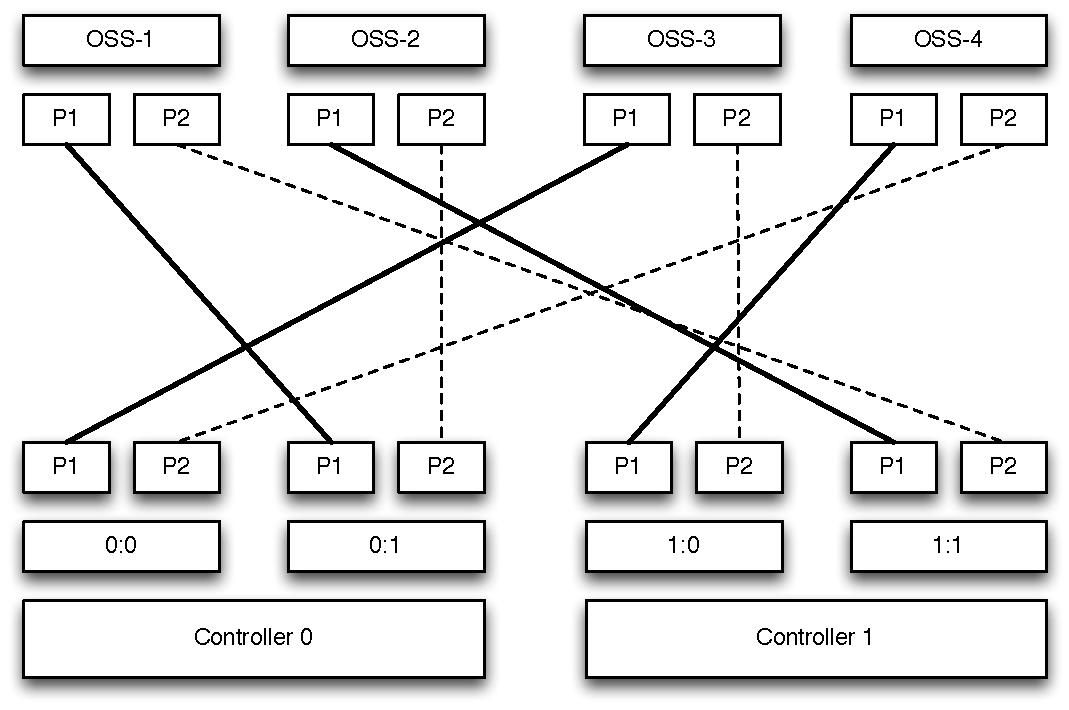
\includegraphics[width=4in]{figs/sfa10k}
\caption{DDN SFA10K Hardware and Host Connection Diagram}
\label{fig:ddn-sfa10k}
\end{figure}


Our Ceph testbed employs a collection of testing nodes. These nodes and their
roles are summarized in Table~\ref{tbl:ceph-test-nodes}. In the following
discussion, we use ``servers'', ``osd servers'', ``server hosts''
interchangably. We will emphasize with ``client'' prefix when we want to
distinguish it from above.

\begin{table}[H]
\centering
    \begin{tabular}{ll}
    \toprule
    Node & Role \\
    \midrule
    tick-mds1 & Ceph monitor node \\
    spoon46 & Ceph MDS node \\
    tick-oss[1-4] & Ceph OSD servers \\
    spoon28-31, spoon37-41 & Ceph client nodes \\
    \bottomrule

    \end{tabular}
\caption{Support nodes involved in Ceph testbed}
\label{tbl:ceph-test-nodes}
\end{table}

All hosts  (client and servers) were configured with Redhat 6.3 and kernel
version 3.5.1 (rhl-ceph image), Glibc 2.12 with syncfs support, locally patched.
We used the Ceph 0.55 release in the initial tests, upgraded to 0.64 and then to
0.67RC for a final round of tests.

%For a complete a list of hosts that are running ceph images, one can execute:

%\begin{Verbatim}
%$ grep "rhel6-ceph" /etc/gedi/MAC.info
%\end{Verbatim}

\section{Baseline Performance}
\label{sec:block-io}

\subsection{Block I/O over Native IB}
We first established baseline performance by measuring observed block I/O
performance.
At the block-level, with each LUN configured as a RAID6 8+2 array, we had the
following results as shown in Table~\ref{tbl:block-io-baseline}.

\begin{table}[htb]
\centering
\begin{tabular}{ll}
    \toprule
    SAS single LUN sequential read & ~1.4 GB/s \\
    SATA single LUN sequential read & ~955 MB/s \\[0.5em]
    Single host with four SAS LUNs & ~ 2.8 GB/s \\
    Single host with seven SATA LUNs & ~ 2.6 GB/s \\
    \bottomrule
\end{tabular}
\caption{Block I/O performances on single LUN and single host}
\label{tbl:block-io-baseline}
\end{table}

Single host in this table refers to one of four tick-oss nodes. Four tick-oss
nodes drive the SFA10K backend storage. Overall, we observe that the entire
system can perform at 11 GB/s, compared to DDN SFA10K's theoretical maximum of
12 GB/s.


\subsection{IP over IB}

Ceph uses the BSD Sockets interface in \texttt{SOCK\_STREAM} mode (i.e., TCP).
Because our entire testbed is IB-switched, we used IP over IB (IPoIB) for
networking\footnote{As of writing of this report, Inktank is investigating using
rsockets to improve performance with IB fabric}. Through simple
\verb!netperf! tests, we observed that a pair of hosts connected by IB QDR using
IPoIB can transfer data at 2.7 GB/s (the hosts are tuned per recommendations
from Mellanox). With all four hosts (OSD servers), we expect the aggregate
throughput to be in the neighborhood of 10 GB/s.

Unfortunately there was not enough time to do more detailed analysis of the network
performance. Later, we will see RADOS is performing a
maximum of 5-6 GB/s driven by four hosts.  So, it shows that we
have enough network bandwidth (i.e., IP over IB is not a bottleneck in this
case).




\section{System Tuning}

Base upon past experience and further experimentation, we started out with the
following set of tuning parameters on OSD servers:

\begin{table}[htb]
\centering
\begin{tabular}{ll}
    \toprule
    \verb!nr_requests! & 2048 \\
    \verb!read_ahead_kb! & 4096 \\
    \verb!scheduler! & deadline \\
    \bottomrule
\end{tabular}
\caption{System tuning parameters}
\end{table}



\section{XFS Performance As Backend File System}

Ceph supports multiple backend file systems including Btrfs, Ext4, and XFS.
Due to its performance and maturity, we chose XFS. We experimented with XFS to
acquire a set of configuration parameters which provided optimal performance for
the SFA10K. We sampled a selected set of parameters (block size, queue depth,
request size, sequential read and write). We settled on the following
configuration: mount with \verb!nobarrier,noatim,inode64! options.
The \verb!inode64! option had a notable improvement on sequential write (around
20\%).

%% Can the graphs be adjusted to have the same values in the Y axis?
\begin{figure}[htb]
\centering
%% -- 1st figure
\centering
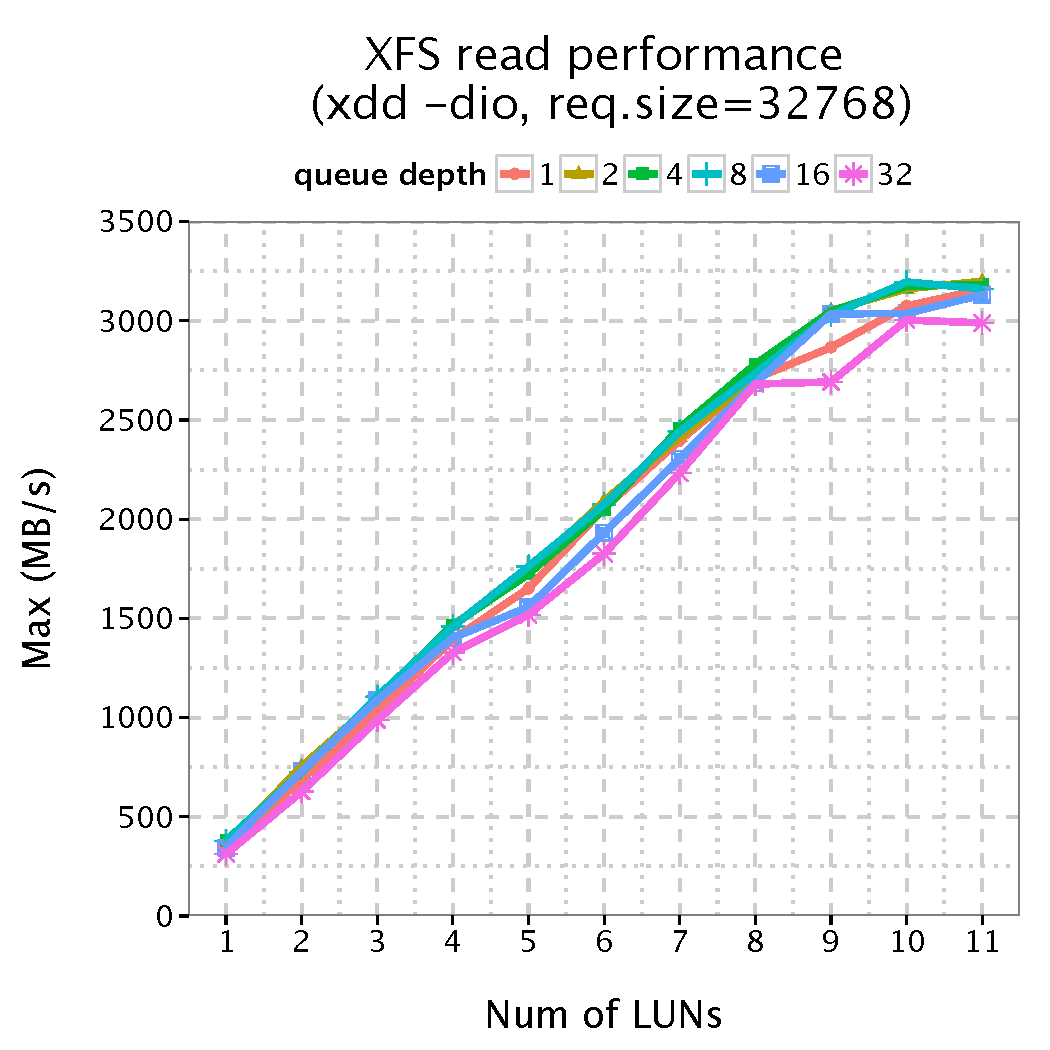
\includegraphics[width=3in]{data/xdd-read}
\caption{XFS read performance scaling on number of devices}
\label{fig:xfs-read}
\end{figure}

\begin{figure}[htb]
\centering
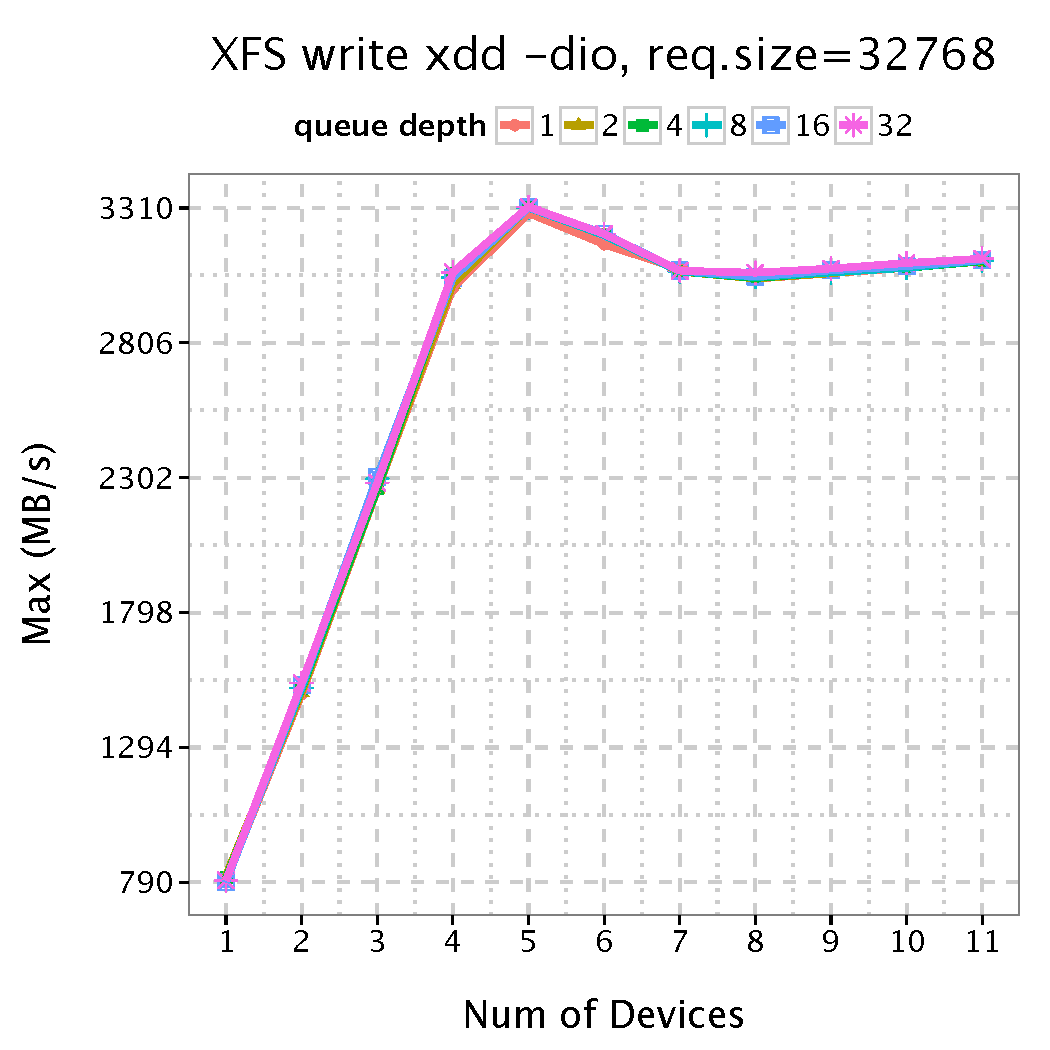
\includegraphics[width=3in]{data/xdd-write}
\caption{XFS write performance scaling on number of devices}
\label{fig:xfs-write}
\end{figure}



%\begin{figure}[htb]
%\centering
%% -- 1st figure
%\begin{minipage}[t]{0.5\linewidth}
%\centering
%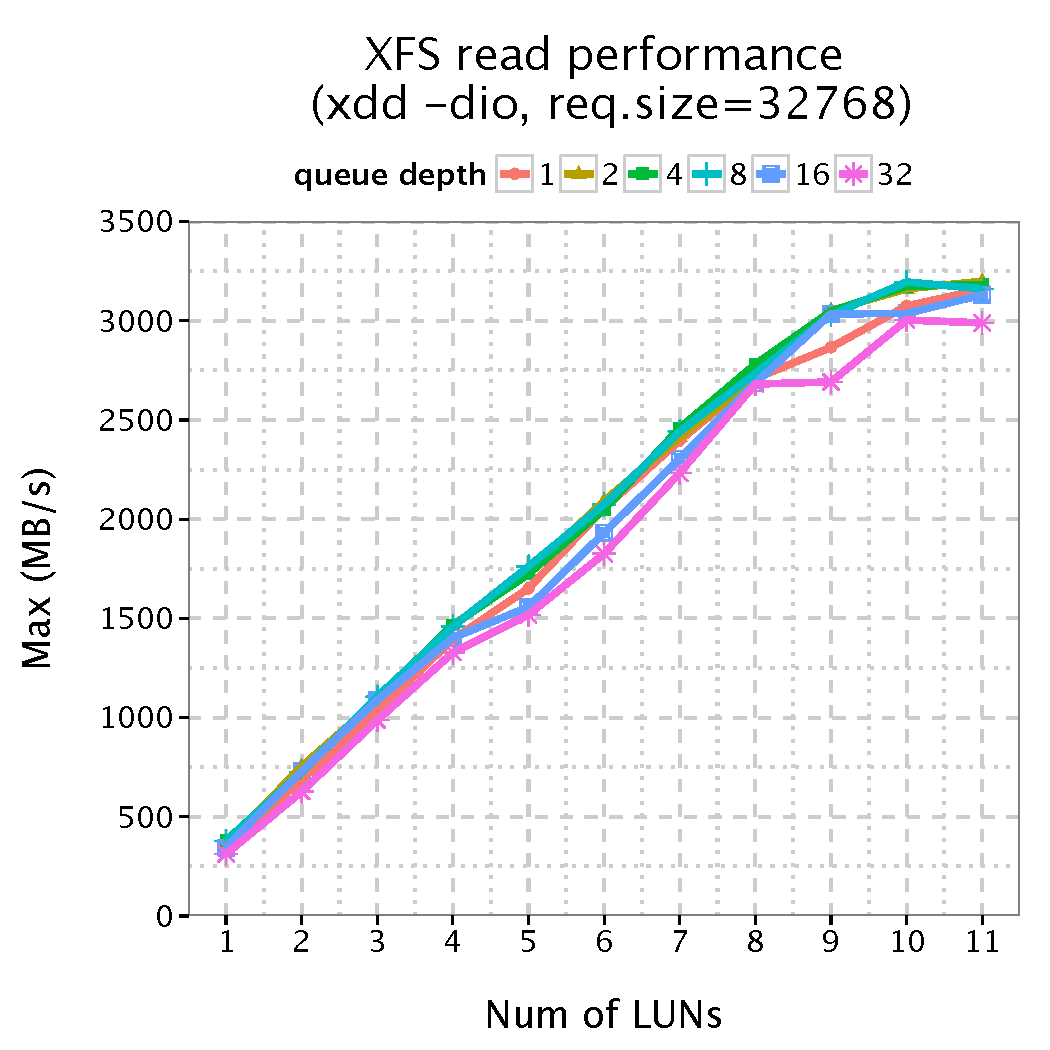
\includegraphics[width=3in]{data/xdd-read}
%\caption{XFS read performance scaling on number of devices}
%\label{fig:xfs-read}
%\end{minipage}%
%\begin{minipage}[t]{0.5\linewidth}
%\centering
%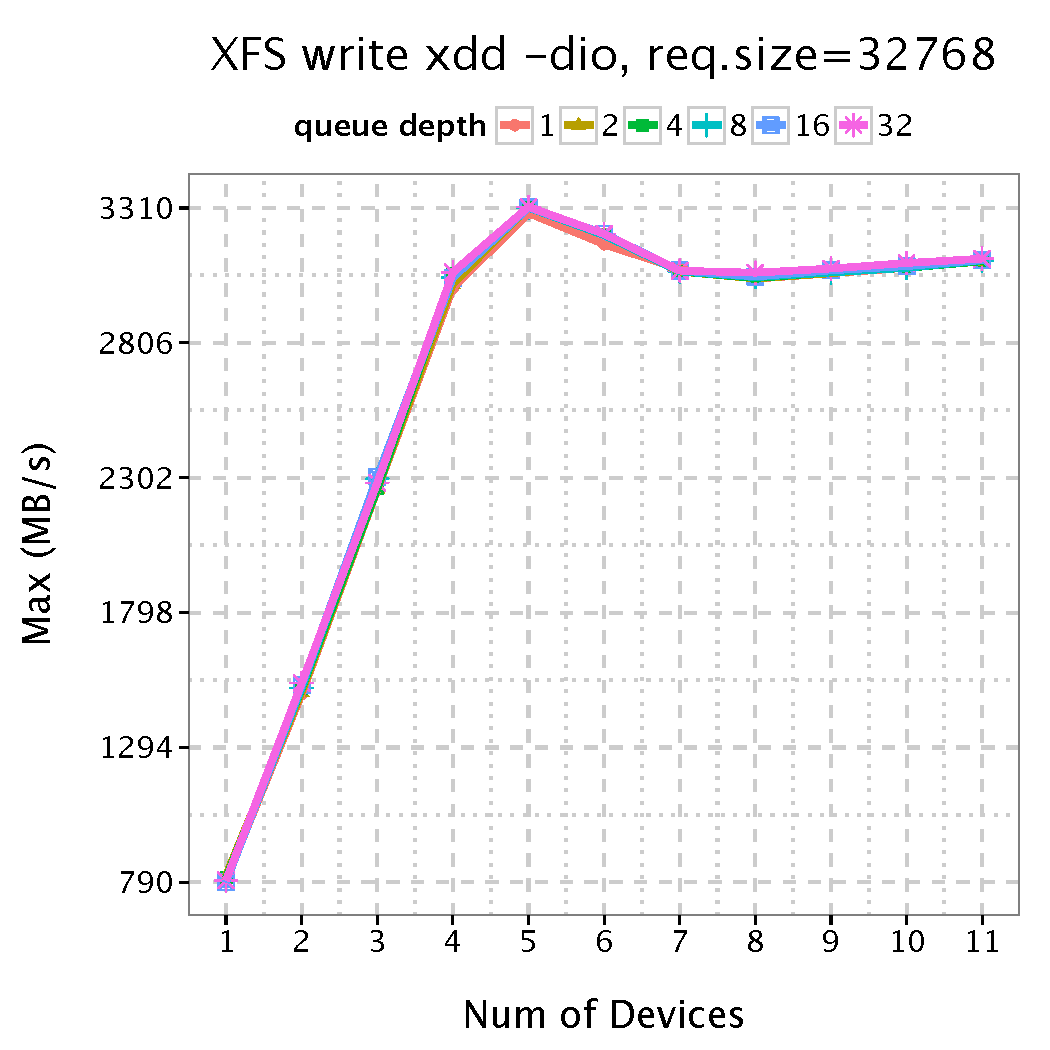
\includegraphics[width=3in]{data/xdd-write}
%\caption{XFS write performance scaling on number of devices}
%\label{fig:xfs-write}
%\end{minipage}%
%\end{figure}



% % Are the read and write graphs wrong or should the second sentence below be
% about write % instead of read?
The read and write performance results are summarized in
Figures~\ref{fig:xfs-read} and~\ref{fig:xfs-write}, respectively. These show
scaling behavior over the number of LUNs, which indicates that XFS can reach
the peak write performance with five SATA LUNs. Increasing number of LUNs
beyond 5, degradation happened. 
Changes to the queue depth was not observed to make any obvious difference in
the performance. For these tests, we used the \verb!xdd! benchmark with direct
I/O and a request size of 32 KB.


\section{Ceph RADOS Scaling: Initial Test}

RADOS is the Ceph object store, the foundational component for CephFS file
system. There are two types of scaling tests we are interested at the RADOS
layer:

\begin{itemize}
  \item scaling on the number of OSD servers
  \item scaling on the number of OSDs per OSD server
\end{itemize}

Our system setup poses some limitations on the scalability tests we wanted to
perform. In particular, we currently had four OSD servers, eight clients, and
eleven OSD servers per client. The scaling tests, therefore, will be within
these constraints.

We used the open-source RADOS Bench tool, developed by Inktank, to perform our
initial performance analysis of the underlying RADOS layer.  RADOS Bench simply
writes out objects to the underlying object storage as fast as possible, and
then later reads those objects in the same order as they were written.

We observed that using two or more client processes and many concurrent
operations are important when performing these tests.  We tested eight client processes 
with 32 concurrent 4 MB objects in flight each. We created a pool for
each RADOS Bench process to ensure that object reads come from independent pools
(RADOS Bench is not smart enough to ensure that objects are not read by multiple
processes and thus possibly cached).  A sync and flush is performed on every
node before every test to ensure no data or metadata is in cache.  All tests
were run with replication set to one.  The backend file systems were XFS,
BTRFS and EXT4 file systems were not tested at this time.


\subsection{Scaling on number of OSDs per server}

In the following test, a single Ceph host drives $n$ OSDs, where $n$ increases
from one to eleven. The result is illustrated in Figure~\ref{fig:osd-scale}.
We ran the test against a single client with four concurrent processes. In this
test case, we observe that the OSD server exhibits near linear scalability up to
nine OSDs, and is still trending upwards at eleven OSDs. This suggests that we
have not reached the saturation point yet. Additional testing would require
provisioning more OSDs on the SFA10K backend.


\begin{figure}[H]
\centering
%% -- 1st figure
\begin{minipage}[t]{0.5\linewidth}
\centering
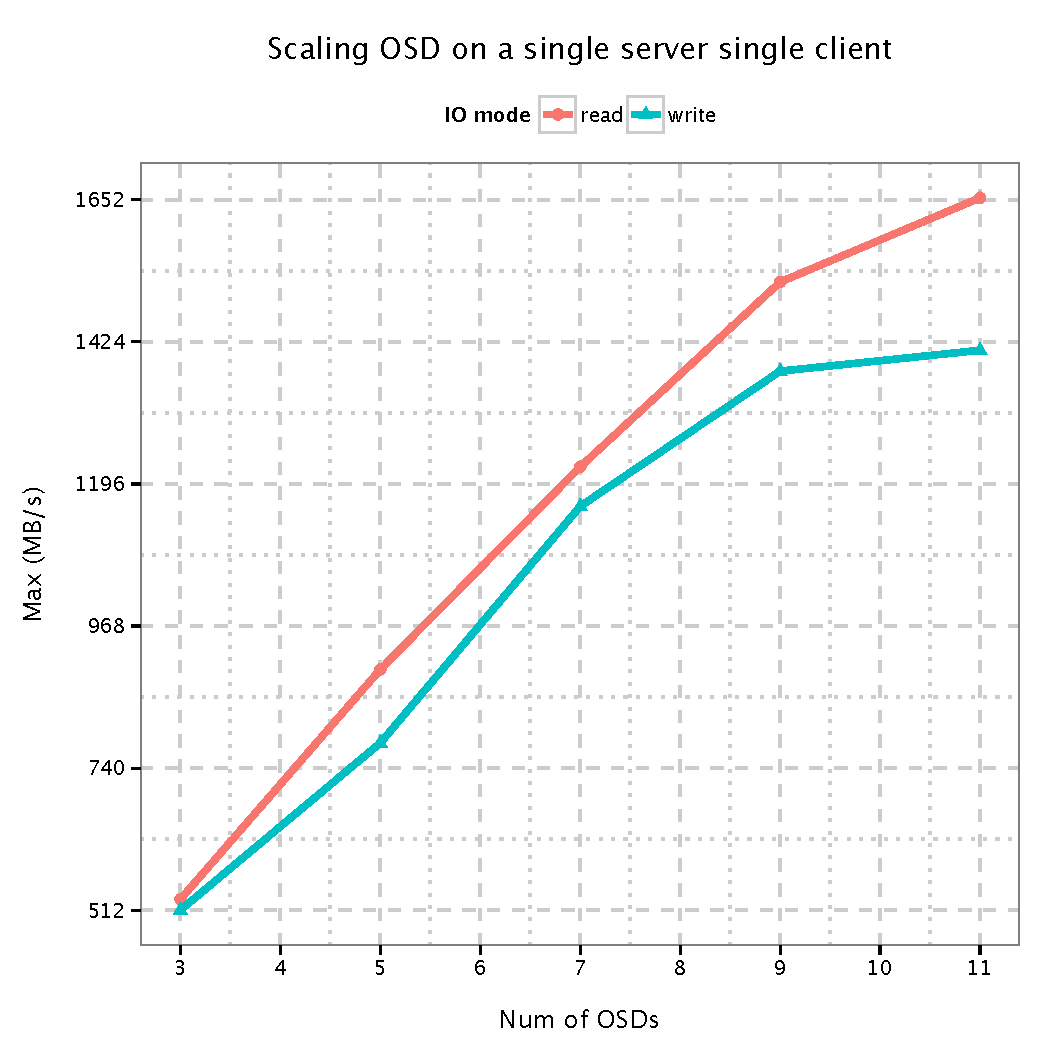
\includegraphics[width=3in]{data/rados_osd}
\caption{RADOS scaling on number of OSDs}
\label{fig:osd-scale}
\end{minipage}%
\begin{minipage}[t]{0.5\linewidth}
\centering
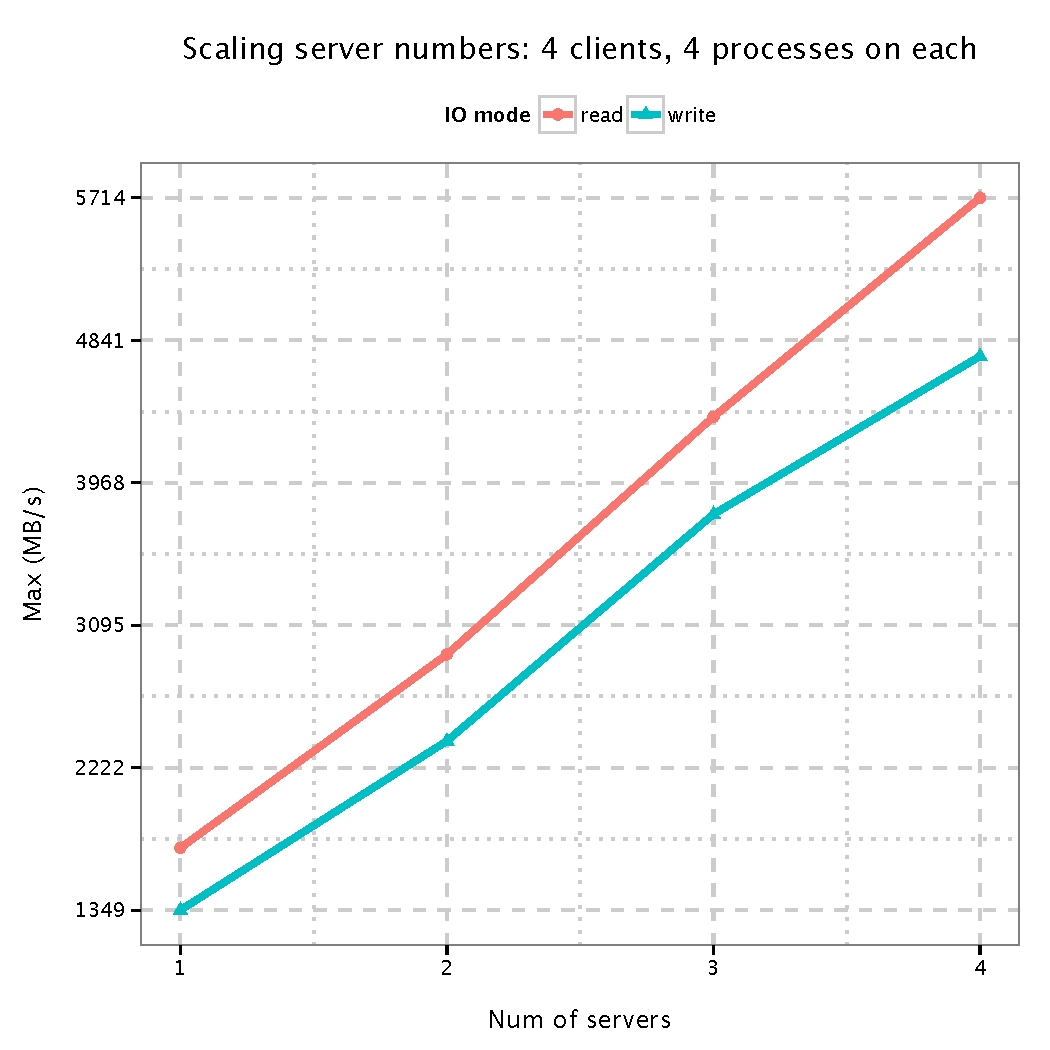
\includegraphics[width=3in]{data/rados_server}
\caption{RADOS scaling on number of servers}
\label{fig:oss-scale}
\end{minipage}%
\end{figure}

\subsection{Scaling on number of OSD servers}

In this test, we exercise OSD servers from one to four, driven by four hosts
each with four RADOS Bench process. Each additional OSD server
adds eleven more OSDs into play. We observe that Ceph exhibits linear scaling with
regard to number of servers as well, at least in the given set of servers.
However, the peak performance we are seeing is about the half of what are
expecting from the SFA10K (compare to the baseline block I/O perforamnce number
presented in Section~\ref{sec:block-io}).

For writes, the lost performance is attributed to the way Ceph performs
journaling:
Ceph does not support meta-data only journaling, therefore every write is the
equivalent of a double-write: once to the data device, once to the journaling
device. This effectively cuts the observed system bandwidth in half. That said,
it does not explain the read performance -- it is a little better than write,
but still far from the theoretical maximum.

\section{Ceph File System Performance: Initial Test}

We used the synthetic IOR benchmark suite for file system level performance and
scalability test.
The particular parameter setup is show in Table \ref{tbl:ior}. Each client node
has 6 GB of physical memory, the block size is set so as to mitigate cache
effects. In addition, the test harness program issues the following commands
at the beginning of each test:




\begin{table}[tb]
\centering
\begin{tabular}{p{1.5in} | p{3in}}
    \toprule
    IOR parameter & Note \\ \midrule
    \verb!-F! & file per process \\ \midrule
    \verb!-a POSIX! & use POSIX API \\ \midrule
    \verb!-w -r -C! & do both write and read test, \verb!-C! is to change task
        ordering for read back so it will not read from the write cache. \\ \midrule
    \verb!-i 3 -d 5! & 3 iterations and delay 5 seconds betewen iterations \\
    \midrule  
    \verb!-e! & perform \verb!fsync()! upon POSIX write close \\ \midrule
    \verb!-b 8g or 16g! & the block size \\ \midrule
    \verb!-t 4k to 4m! & the transfer size \\ \midrule
    \verb!-o file! & mandatory test file  \\    
    \bottomrule
\end{tabular}
\caption{IOR parameter setup}
\label{tbl:ior}
\end{table}


\begin{Verbatim}
# sync
# echo 3 | tee /proc/sys/vm/drop_caches
\end{Verbatim}


Here, 0 is the default value of \verb!drop_caches!; 1 is to free pagecaches, 2
is to free dentries and inodes, 3 is to free pagecache, dentries, and inodes.


Our first round of tests was less than ideal as we encountered various issues. For
the sake of completeness, we first summarize the results, then discuss
further tuning efforts and improvements.

The full permutation of IOR parameters were not explored due to I/O errors we encountered.
We were, however, able to record results in two extreme cases as far as
transfer size is concerned: 4 KB and 4 MB, using a fixed number of OSD servers
(4) and fixed block size (8 GB), the results are illustrated in Figure
\ref{fig:ior4k} and \ref{fig:ior4m}, we make the following observations:

%% SCOTT - figures 4-7 do not seem to use a base of 0 for the Y axis. Is this common?
%% SCOTT - Can figures 6-7 have the same Y axis with either base 2 or base 10 values?

%% FEIYI: 6, 7 all fixed.

\begin{figure}[H]
\centering
%% -- 1st figure
\begin{minipage}[t]{0.5\linewidth}
\centering
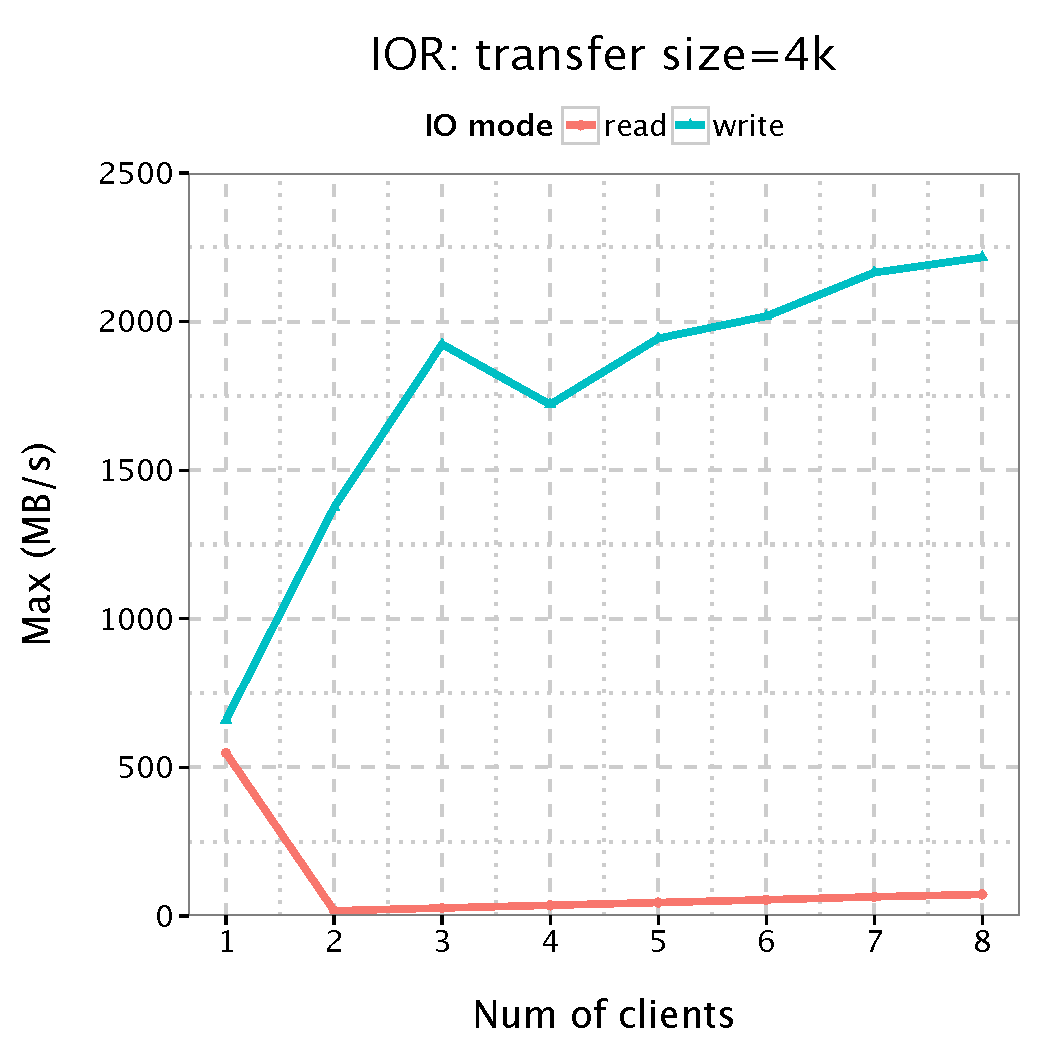
\includegraphics[width=3in]{data/ior_4k}
\caption{IOR tests: 4 KB transfer size}
\label{fig:ior4k}
\end{minipage}%
\begin{minipage}[t]{0.5\linewidth}
\centering
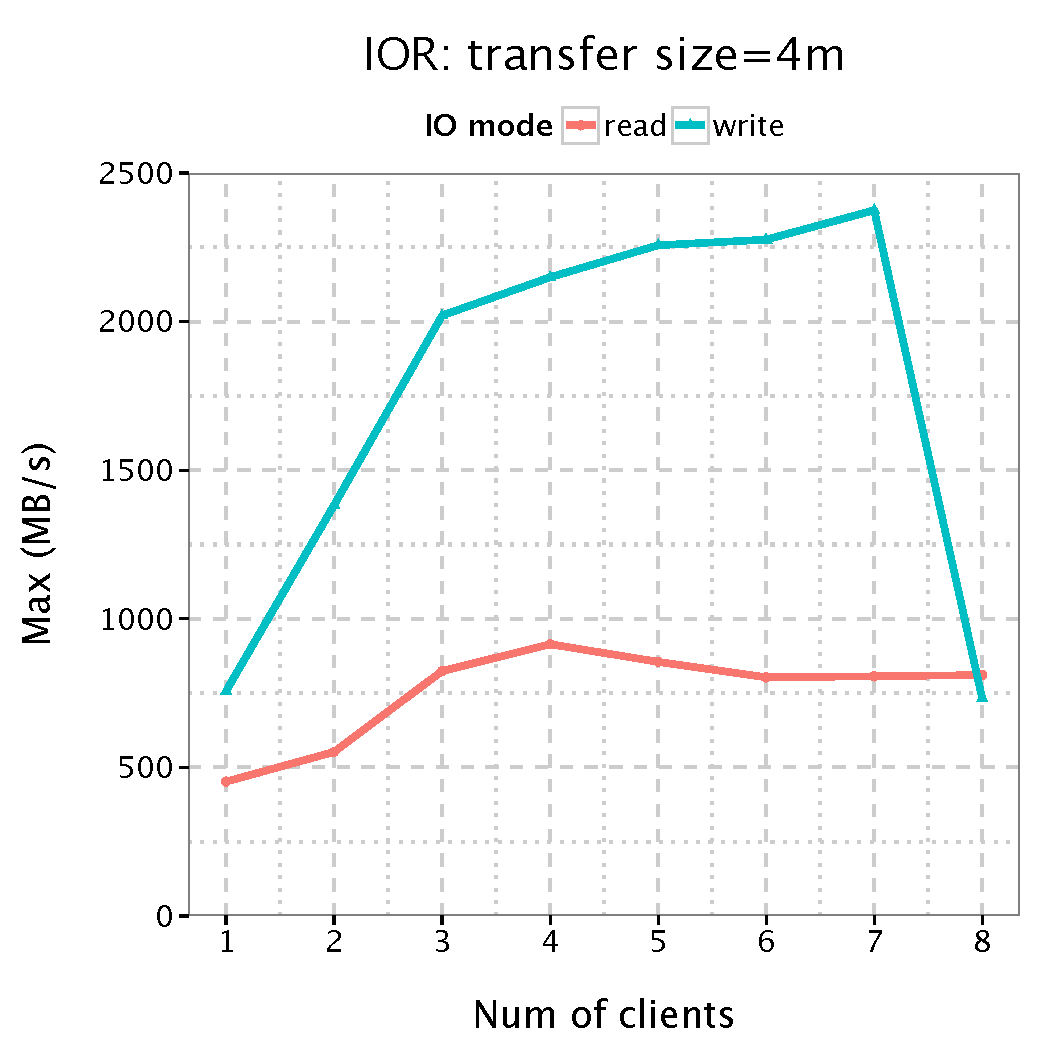
\includegraphics[width=3in]{data/ior_4m}
\caption{IOR tests: 4 MB transfer size}
\label{fig:ior4m}
\end{minipage}%
\end{figure}


\begin{itemize}
  \item The small read (4 KB transfer size) performance is almost an anomaly --
  we will investigate why it is so low compare to write performance and improved
  results in Section~\ref{sec:improve-ior}.
  \item The large read (4 MB transfer size) performance is almost half of the
  RADOS read performance.
   
  \item The write performance is also about half of what we can obtain from
  RADOS Bench. When number of clients reaches 8, there is a significant
  performance drop as well. 
\end{itemize}


%\begin{figure}[htb]
%\centering
%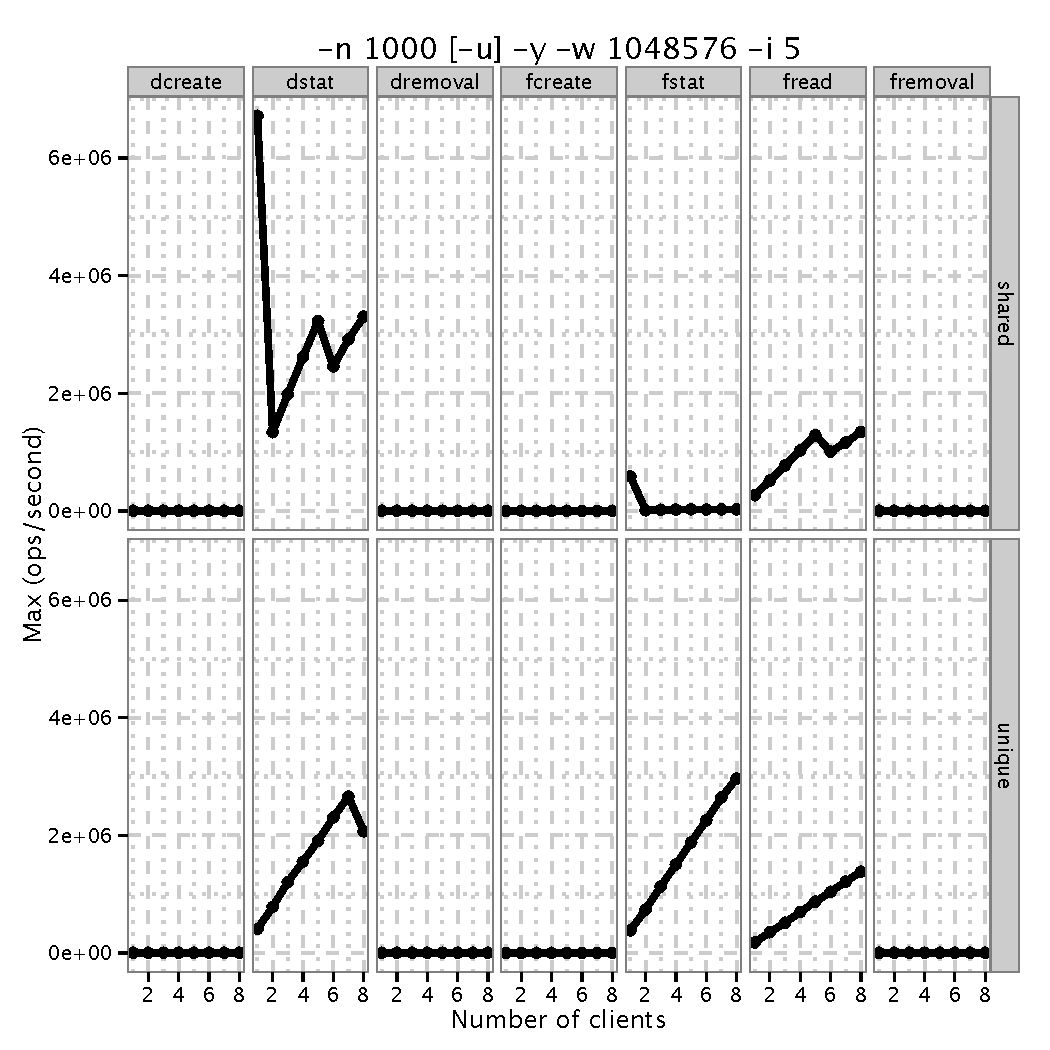
\includegraphics[width=5in]{data/mdtest}
%\caption{mdtest of single MDS}
%\label{fig:mdtest1c}
%\end{figure}

We will describe the efforts and results on performance improvement in the
following sections.

\section{Improving RADOS Performance}

\begin{figure}[h]
\centering
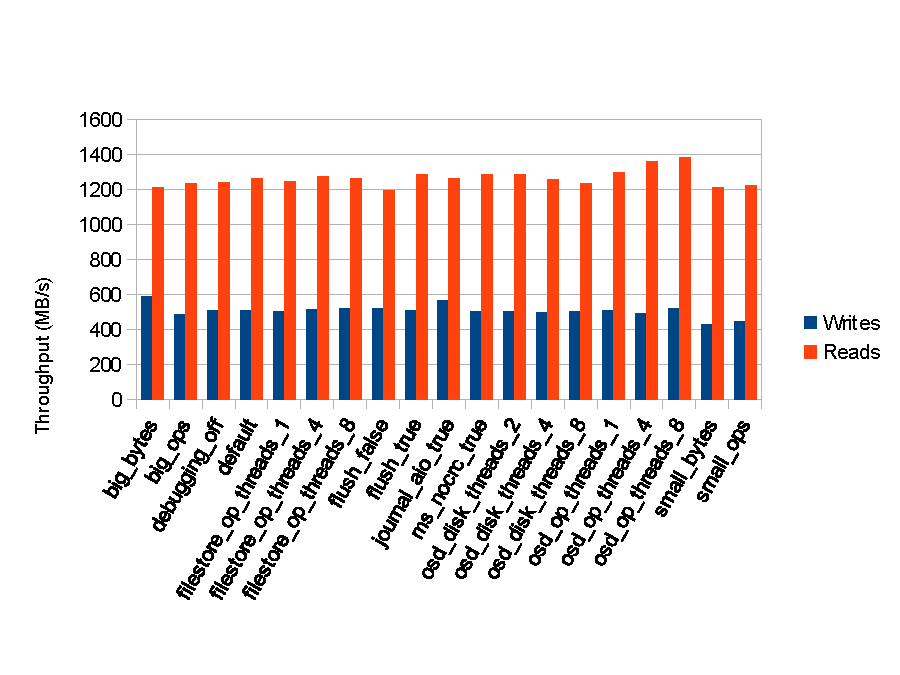
\includegraphics[width=5in]{parametric}
\caption{Evaluating parameter impact through sweeping test}
\label{fig:parametric}
\end{figure}


After the initial test results, we tried various combinations of tweaks
including changing the number of filestore op threads, putting all of the
journals on the same disks as the data, doubling the OSD count, and upgrading
Ceph to a development version which reduces the seek overhead caused by
\texttt{pginfo} and \texttt{pglog} updates on XFS (these enhancements are now
included as of the Ceph Cuttlefish release, v0.61).  The two biggest
improvements resulted from disabling CRC32c checksums and increasing the OSD
count on the server.  With these changes, we are seeing better results.

We ran a script written by Inktank for internal Ceph testing to perform
sweeps over Ceph configuration parameters to examine how different
tuning options affect performance on the DDN platform. The result of this
parameter probing is illustrated in Figure~\ref{fig:parametric}. Please refer
to Appendix E for explanations of these probed parameters.


As a result of this testing, we improved performance slightly by
increasing the size of various Ceph buffers and queues, enabling AIO journals,
and increasing the number of OSD op threads.


\subsection{Disable Cache Mirroring on controllers}

During a second round of test performed by Inktank, we noticed a dramatic drop
on RADOS performance: even though write throughput on individual server met the
expectation, it did not scale across servers.

We spent a significant amount of time
investigating this phenomenon. Ultimately, we were able to replicate this finding
when running concurrent disk throughput tests directly on the servers without
Ceph involved. The second RAID processor on each DDN controller would max out when
three or more LUNs were written concurrently. It turns out the root of the problem
was a regression on DDN firmware update -- in particular, the cache
mirroring was not behaving as it should.\footnote{DDN recently released a new
firmware version and we were told the issue has been fixed. Unfortunately, we didn't get
a chance to verify it during our test cycle.}

%% SCOTT - is running with cache mirroring off and option for a production system or not?
%% What are the consequences? Did DDN eventually provide a fix? If yes, were we able to test
%% with it or not?

%% FEIYI: add footnote to clarify the issue.

\begin{figure}[htb]
\centering
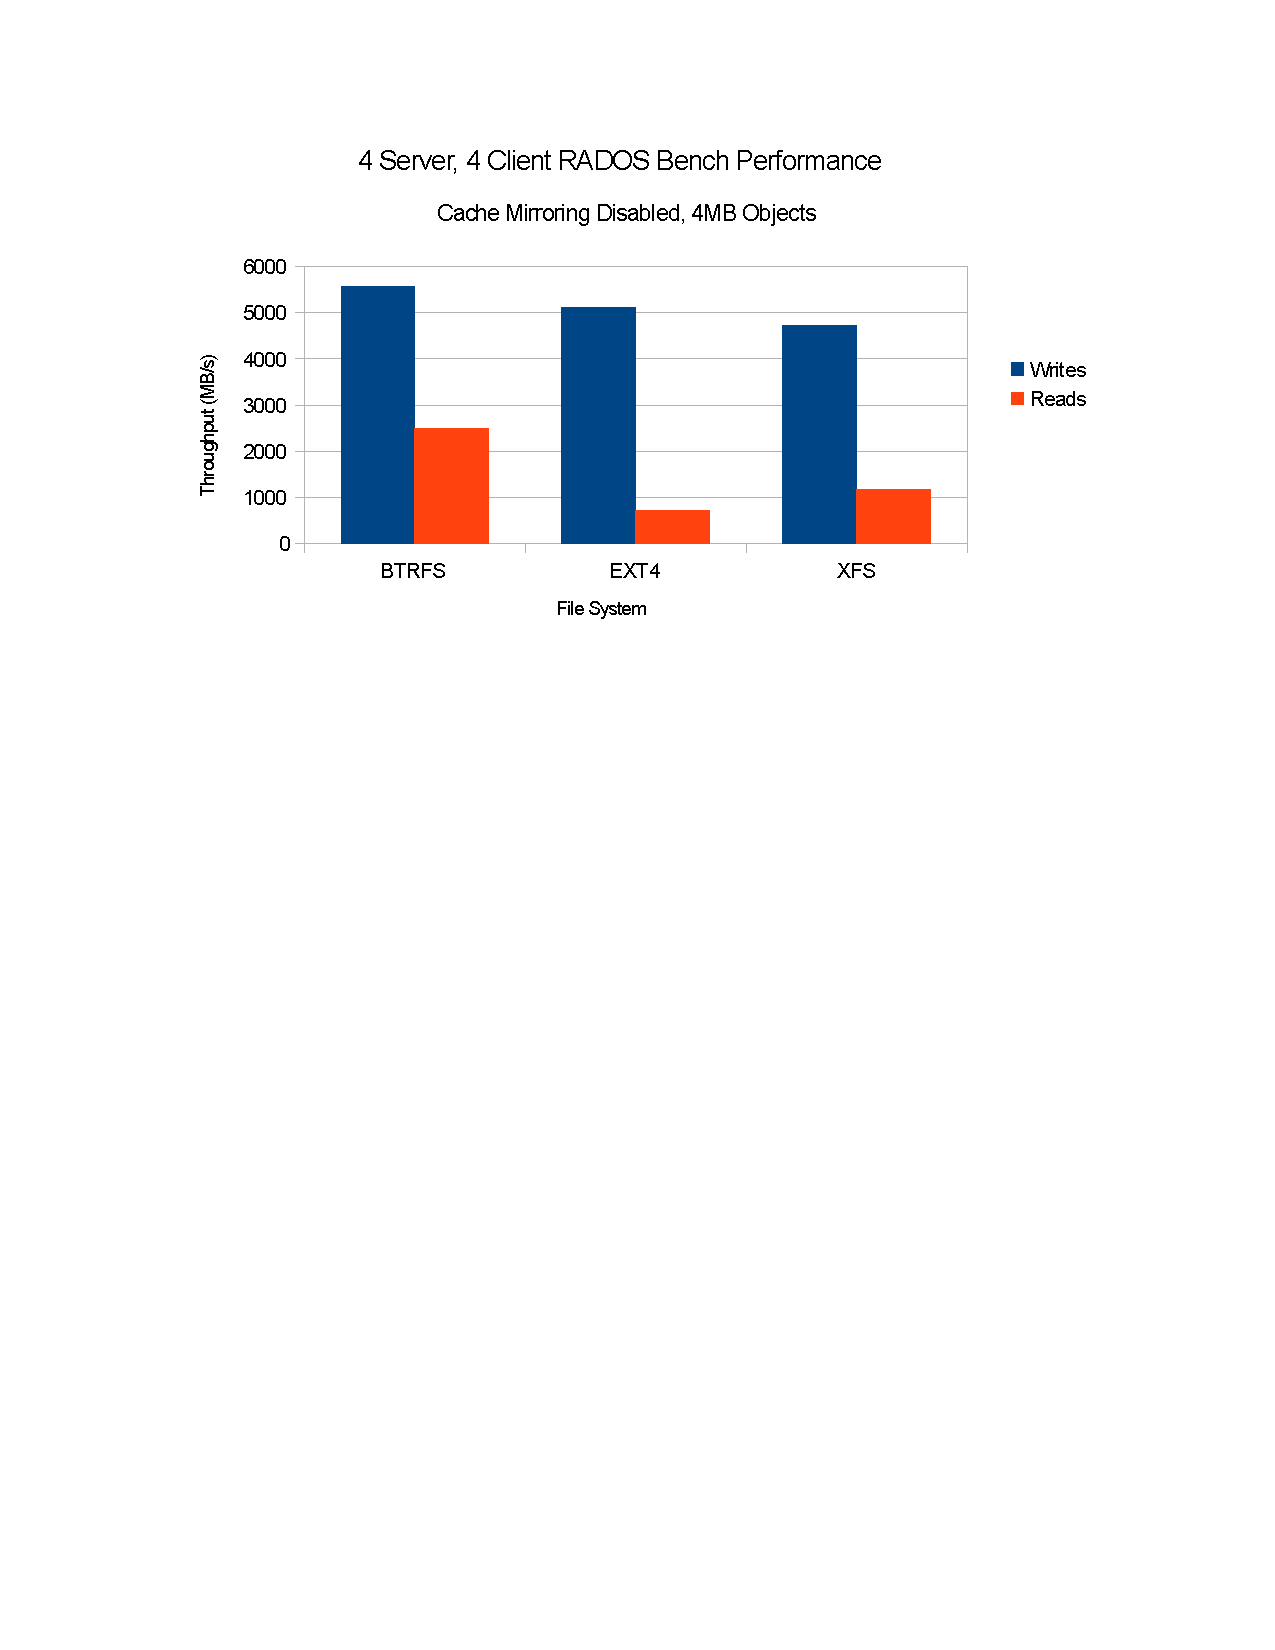
\includegraphics[width=4in]{rados-after-ddn}
\caption{Evaluating RADOS bench after disabling cache mirroring}
\label{fig:rados-ddn-mirror-disabled}
\end{figure}


With cache mirroring disabled, write performance when using all four servers
improved dramatically, as illustrated in
Figure~\ref{fig:rados-ddn-mirror-disabled}. With BTRFS, for example, we hit over
5.5 GB/s from the clients.  When accounting for journal writes, that is over
11 GB/s to the disks and very close to what the DDN chassis is capable of doing. 
Unfortunately, read performance did not scale as well.


\subsection{Disable TCP autotuning}

During these tests, a trend that previously had been seen became more apparent.
During reads, there were periods of high performance followed by periods of low
performance or outright stalls that could last for up to 20 seconds at a time.
After several hours of diagnostics, Inktank observed that outstanding operations
on the clients were not being shown as outstanding on the OSDs.  This appeared
to be very similar to a problem Jim Schutt at Sandia National labs encountered
with TCP autotuning in the Linux Kernel.\footnote{\url{http://marc.info/?l=ceph-devel&m=133009796706284&w=2}}
TCP auto tuning enables TCP window scaling by default and automatically adjusts
the TCP receive window for each connection based on link conditions such as
bandwidth delay product. We have observed this will make a notable improvement
on Ceph read performance, as the results shown in
Figure~\ref{fig:rados-tcp-auto-disabled}.


Luckily, the fix was fairly straight forward by issuing the following command on all nodes:

\begin{Verbatim}
     echo 0 | sudo tee /proc/sys/net/ipv4/tcp_moderate_rcvbuf
\end{Verbatim}

Recent versions of Ceph work around this issue by manually controlling the TCP
buffer size.  The testing at ORNL directly influenced and motivated the creation
of this feature!

\begin{figure}[htb]
\centering
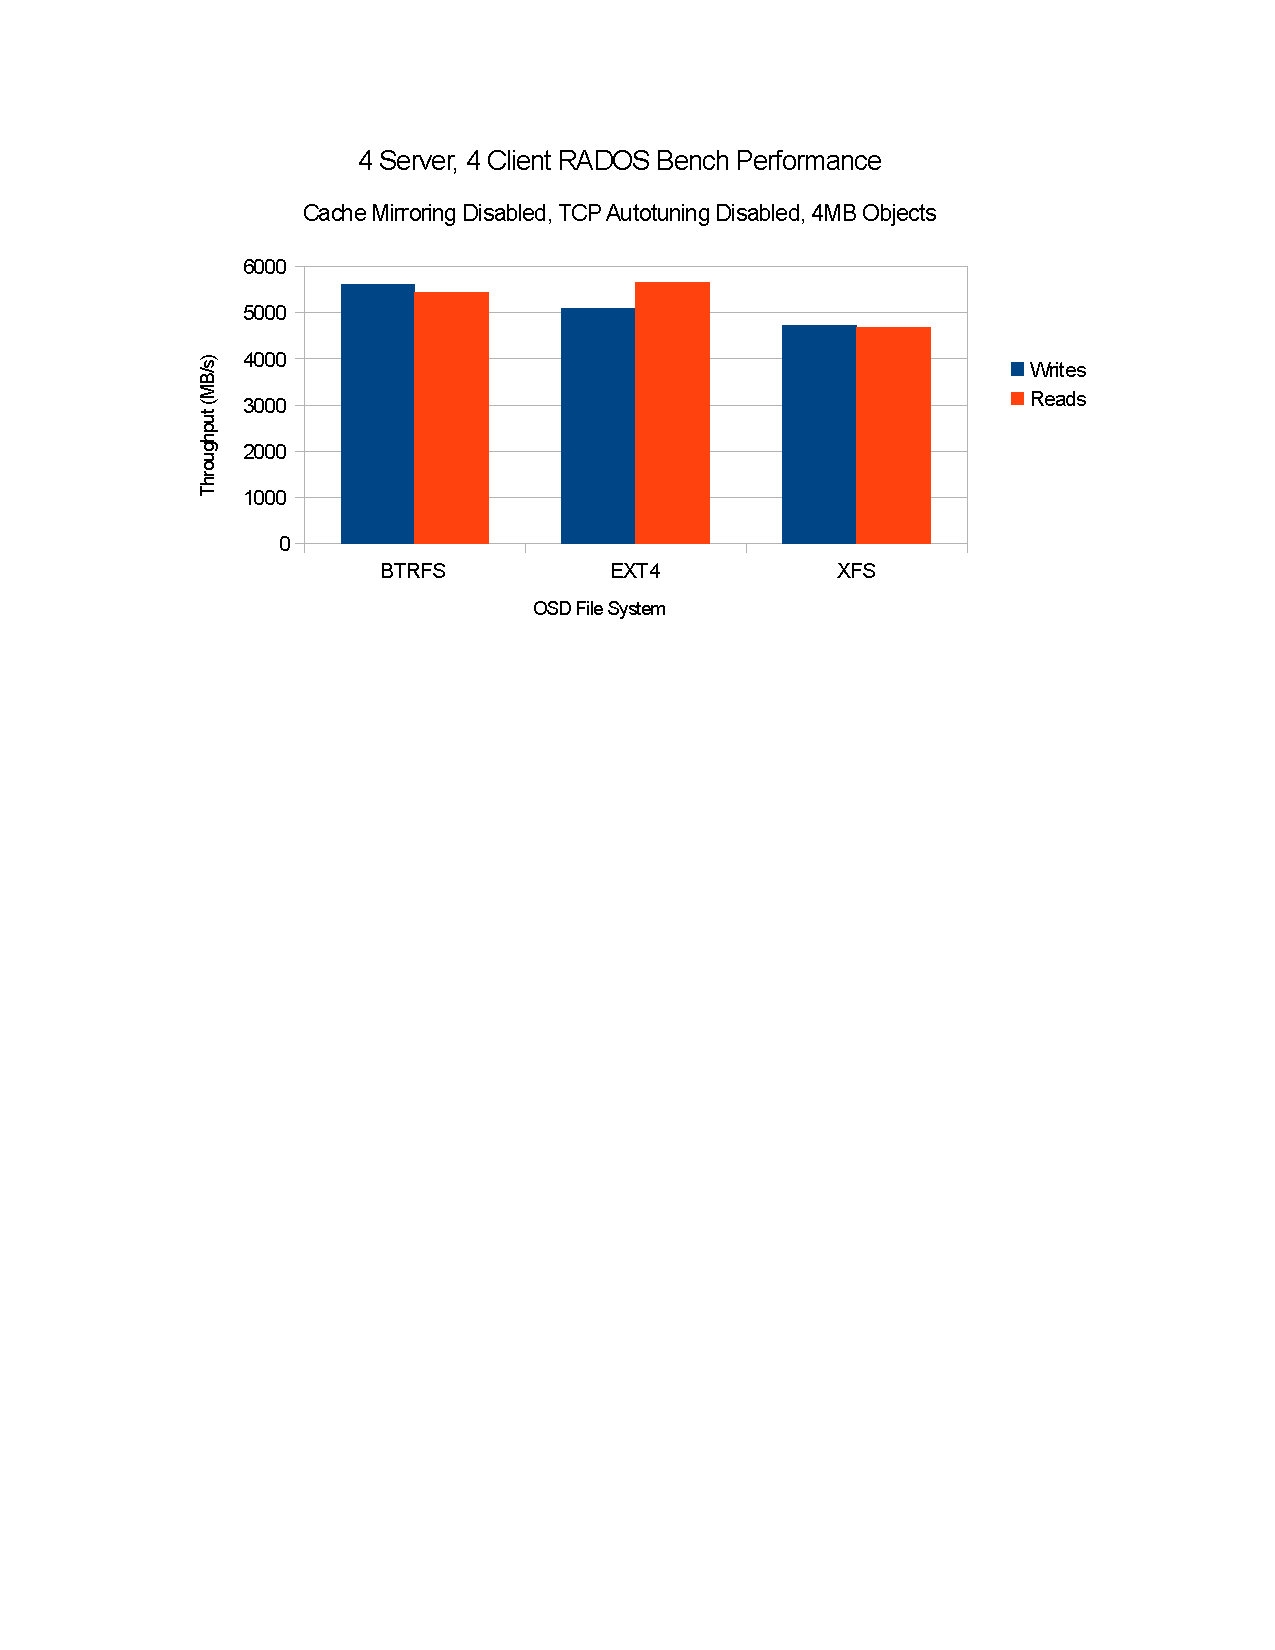
\includegraphics[width=4.0in]{rados-after-ddn-tcptune}
\caption{Evaluating RADOS bench after TCP auto tuning disabled}
\label{fig:rados-tcp-auto-disabled}
\end{figure}



%\begin{figure}[htb]
%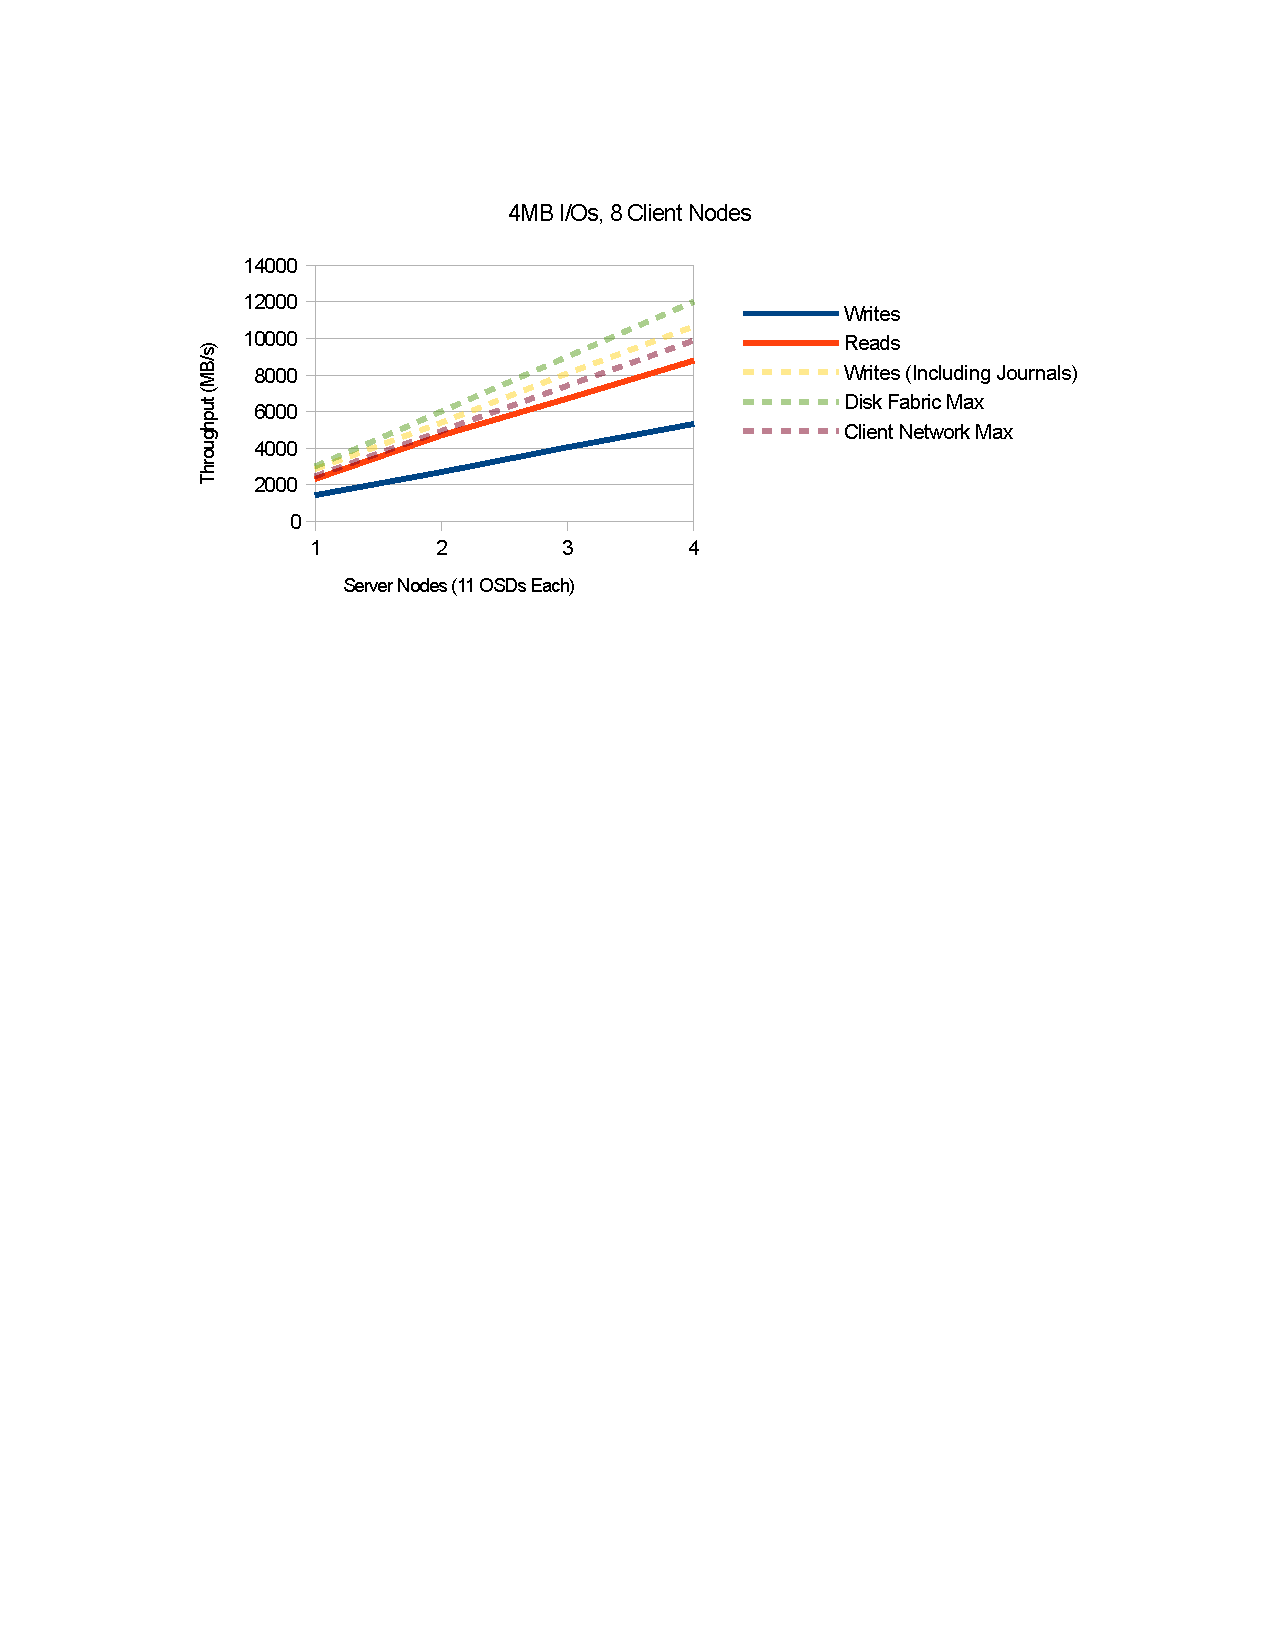
\includegraphics[width=5in]{rados-064-oss}
%\end{figure}

\subsection{Repeating RADOS Scaling Test}

We now repeated the previous RADOS scaling tests with these improvements in place.
The first test was done on a single node with RADOS Bench to see how close the
underlying object store could get to the node hardware limitations as the number
of OSDs/LUNs used on the node increased. Note all the tests performed were against
XFS-formatted storage.

%% SCOTT - the title in the figure needs to change IO to I/O

%% SCOTT - how do writes inc. journals exceed the client network max? Dual ports
%% on the single server?

\begin{figure}[htb]
\centering
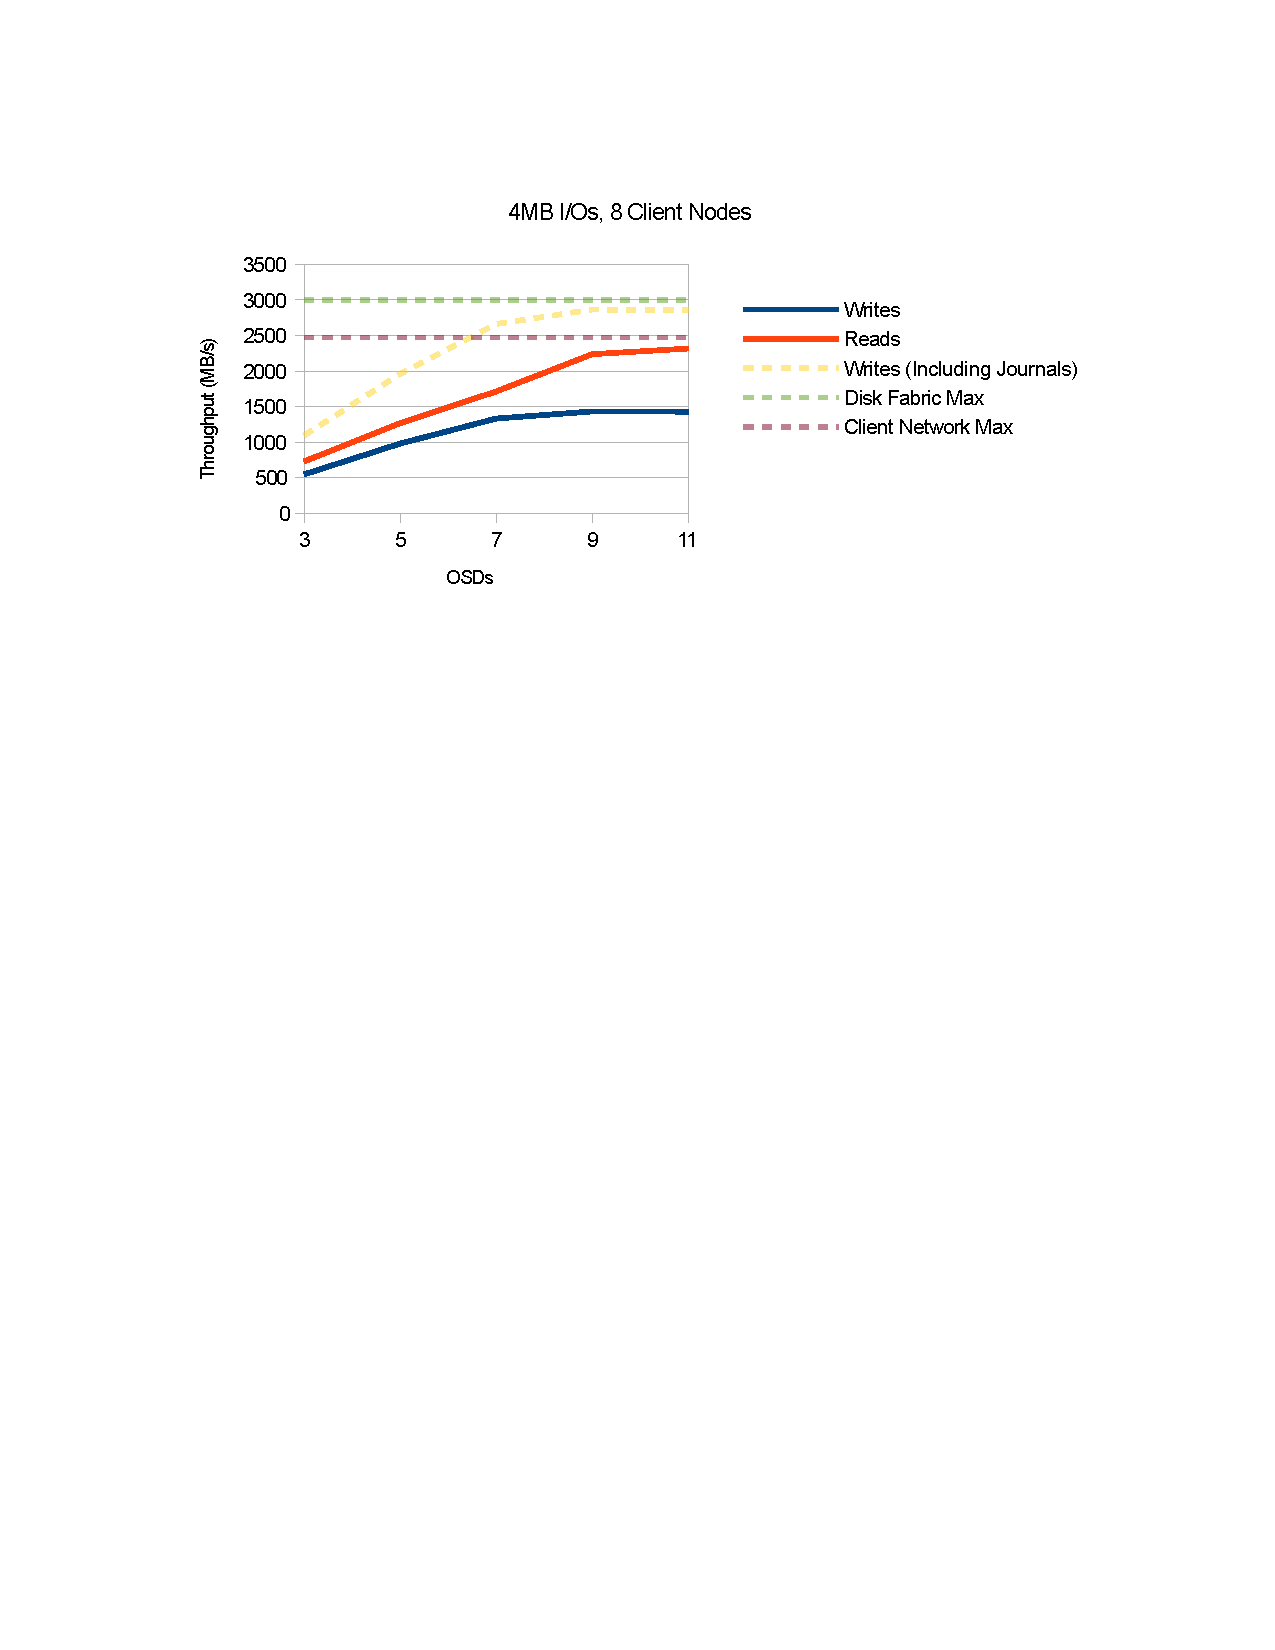
\includegraphics[width=5in]{rados-064-osd}
\caption{RADOS Bench Scaling on \# of OSD, Ceph 0.64, 4 MB I/O, 8 Client Nodes}
\label{fig:rados-064-osd}
\end{figure}

In the single server case as shown in Figure~\ref{fig:rados-064-osd}, ``Writes
(including Journals)'' refers to how much data is actually being written out the
DDN chasis, and blue line is how much data the clients are writing.
We observe that performance gets very close to the hardware limits at roughly 9
OSDs per server and then mostly levels out.

We also repeated tests looking at RADOS Bench performance as the number of OSD
server nodes increases from one to four. The results are summarized in
Figure~\ref{fig:rados-064-oss}. As the number of nodes increases, performance
scales nearly linearly for both reads and writes.

%% SCOTT - why does the client network max scale in figure 12 but not figure 11?
%% Do they no measure the same thing (i.e. a single server)? If not, the text
%% needs to make it more clear.

\begin{figure}[htb]
\centering
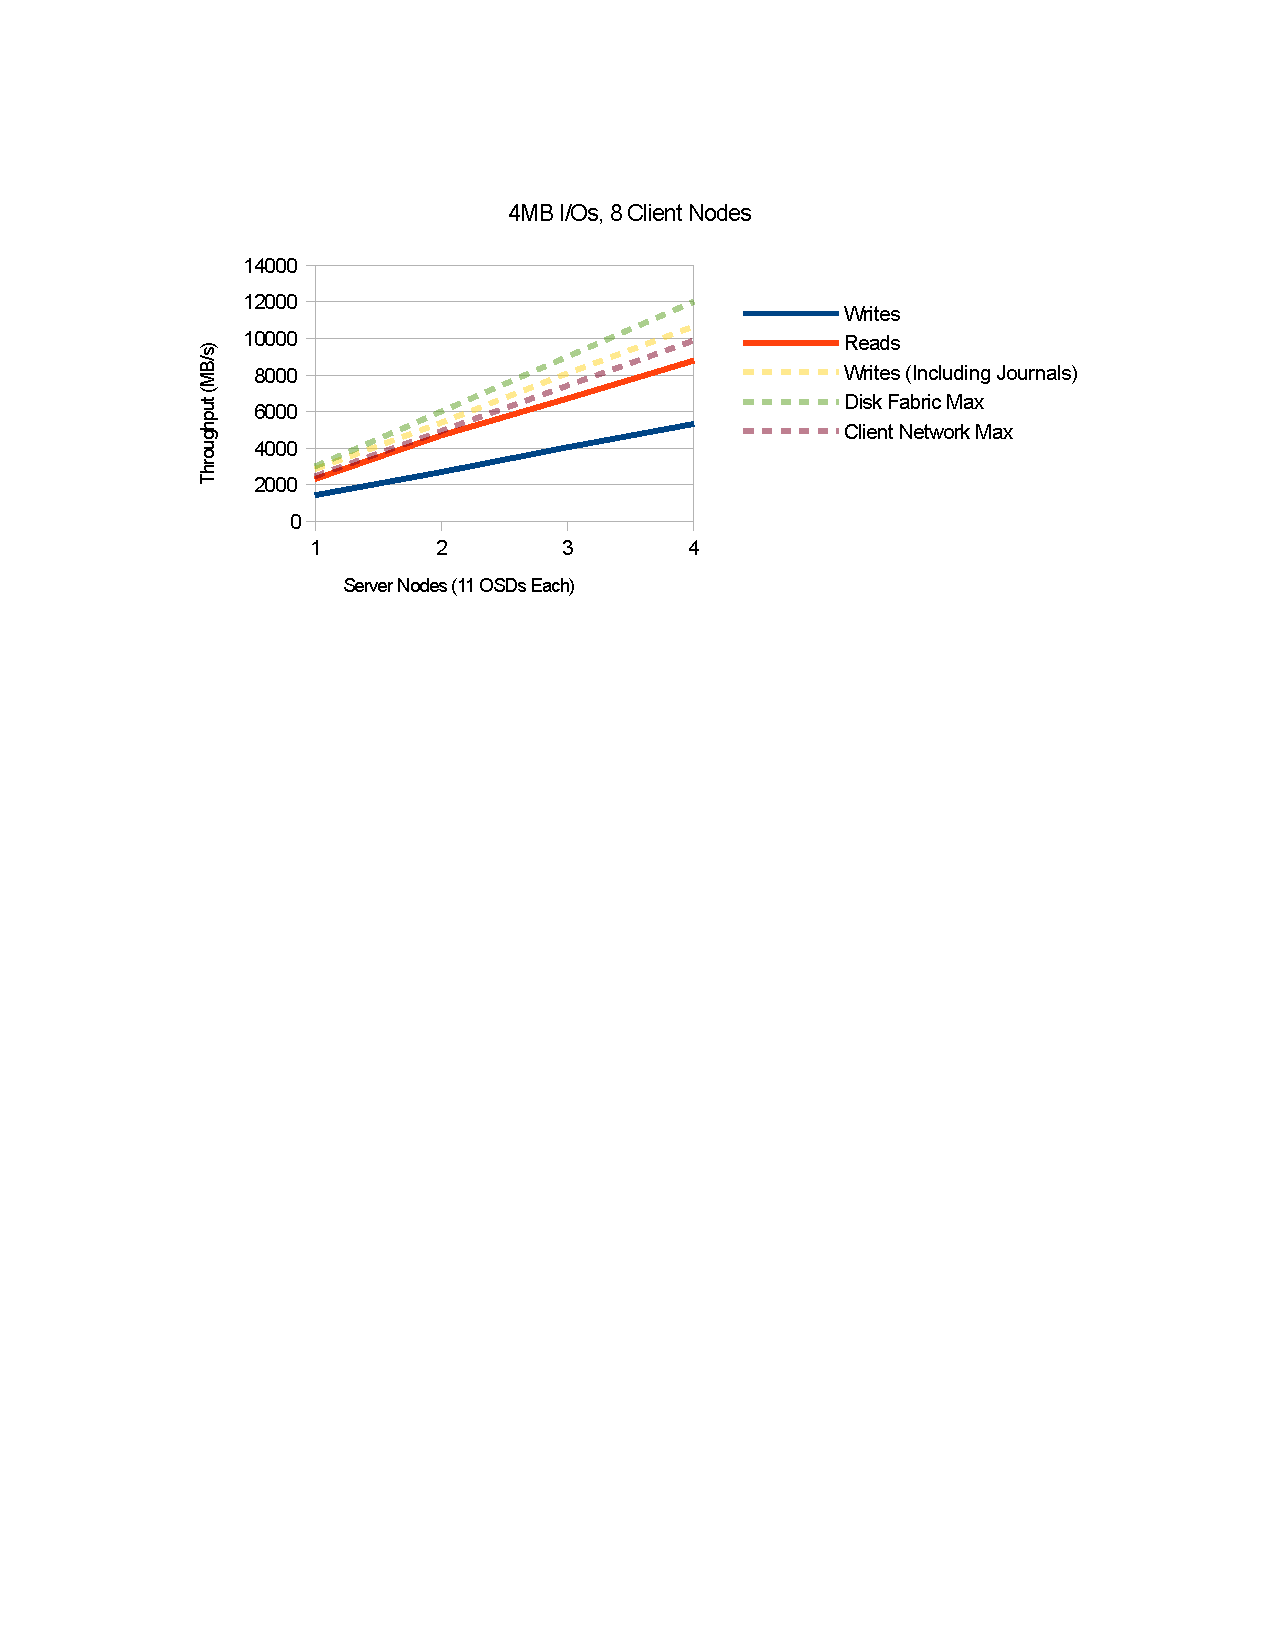
\includegraphics[width=5in]{rados-064-oss}
\caption{RADOS Bench Scaling on number of servers, Ceph 0.64, 4 MB I/O, 8 client
nodes}
\label{fig:rados-064-oss}
\end{figure}



\section{Improving Ceph File System Performance}
\label{sec:improve-ior}

The initial stability issues we encountered are fixed by moving from Ceph
version 0.48/0.55 to 0.64, the latest stable version at the time. Now IOR test
could complete even during long runs. This is another sign of how much Ceph
development is in flux.

Another fix comes in the way we create the pool: the default data pool being used
by previous CephFS cluster are set to 2x replication, which can potentially
halve the write performance. Even with these changes in place, Inktank still
reproduced the less-than-ideal write performance and very poor read
performance as observed by ORNL.  Further, by increasing the number of IOR
processes per client node, read performance actually degraded further
indicating some kind of contention either on the clients or on the OSD
servers.


\subsection{Disabling Client CRC32}

ORNL at this point was able to both make more client nodes available and also
install a profiling tool called \verb!perf! that is extremely useful for
profiling both kernel and user space code.  Profiling with \verb!perf! showed
high CPU utilization on the client due to crc32c processing in the Ceph kernel
client.  Luckily, crc32 checksums can be disabled by changing the CephFS mount
options:

\begin{Verbatim}
mount -t ceph 10.37.248.43:6789:/ /mnt/ceph -o name=admin,nocrc
\end{Verbatim}


With client CRC32 disabled, we repeated the IOR test and the results are showin
in Figure~\ref{fig:ior-no-client-crc32}. 

\begin{figure}[htb]
\centering
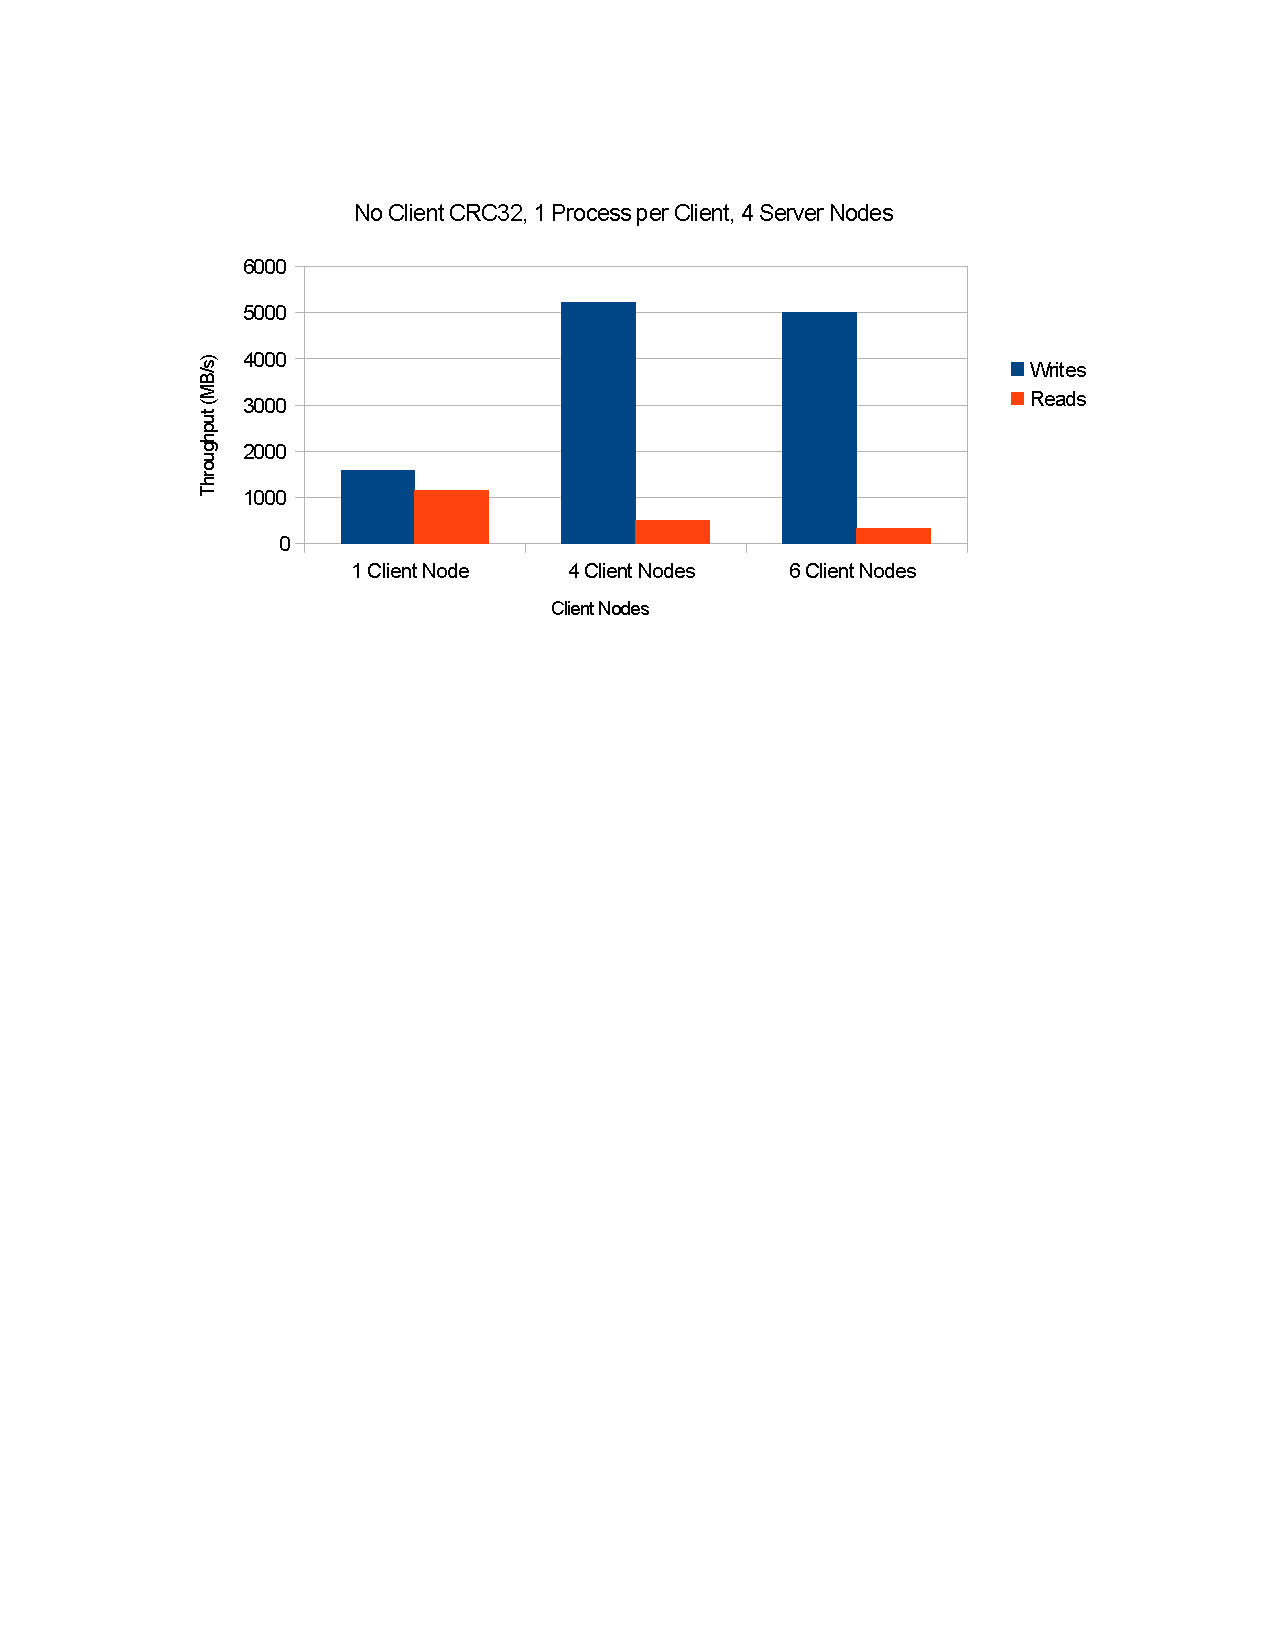
\includegraphics[width=4in]{ior-client-no-crc32}
\caption{IOR test with disabling client-side CRC32}
\label{fig:ior-no-client-crc32}
\end{figure}

We observed that IOR write throughput increased dramatically and is now very
close to the throughput we were able to achieve with RADOS Bench, but reads
continued to be slow and continued to scale inversely with the number of client
processes.  Please note that since these tests were performed, Inktank has
implemented SSE4-based CRC32 code for Intel CPUs.  While any kernel based CRC32
processing should have already been using SSE4 instructions on Intel CPUs, this
will allow any user-land Ceph processes to process CRC32 checksums with
significantly less overhead.

\subsection{Improving IOR Read Performance}

Deeper analysis with perf showed that there was heavy lock contention during
parallel compaction in the Linux kernel memory manager.  This behavior was first
observed roughly in the kernel 3.5 time frame which happens to be the kernel
that ORNL had installed on the test systems.\footnote{For more information,
please refer to \url{http://lwn.net/Articles/517082/} and
\url{https://patchwork.kernel.org/patch/1338691/}.}

ORNL installed kernel 3.9 on all of the test systems and Inktank performed a
RADOS Bench test to verify that there was no degradation versus previous tests.  The
results were extremely positive.


\begin{figure}[htb]
\centering
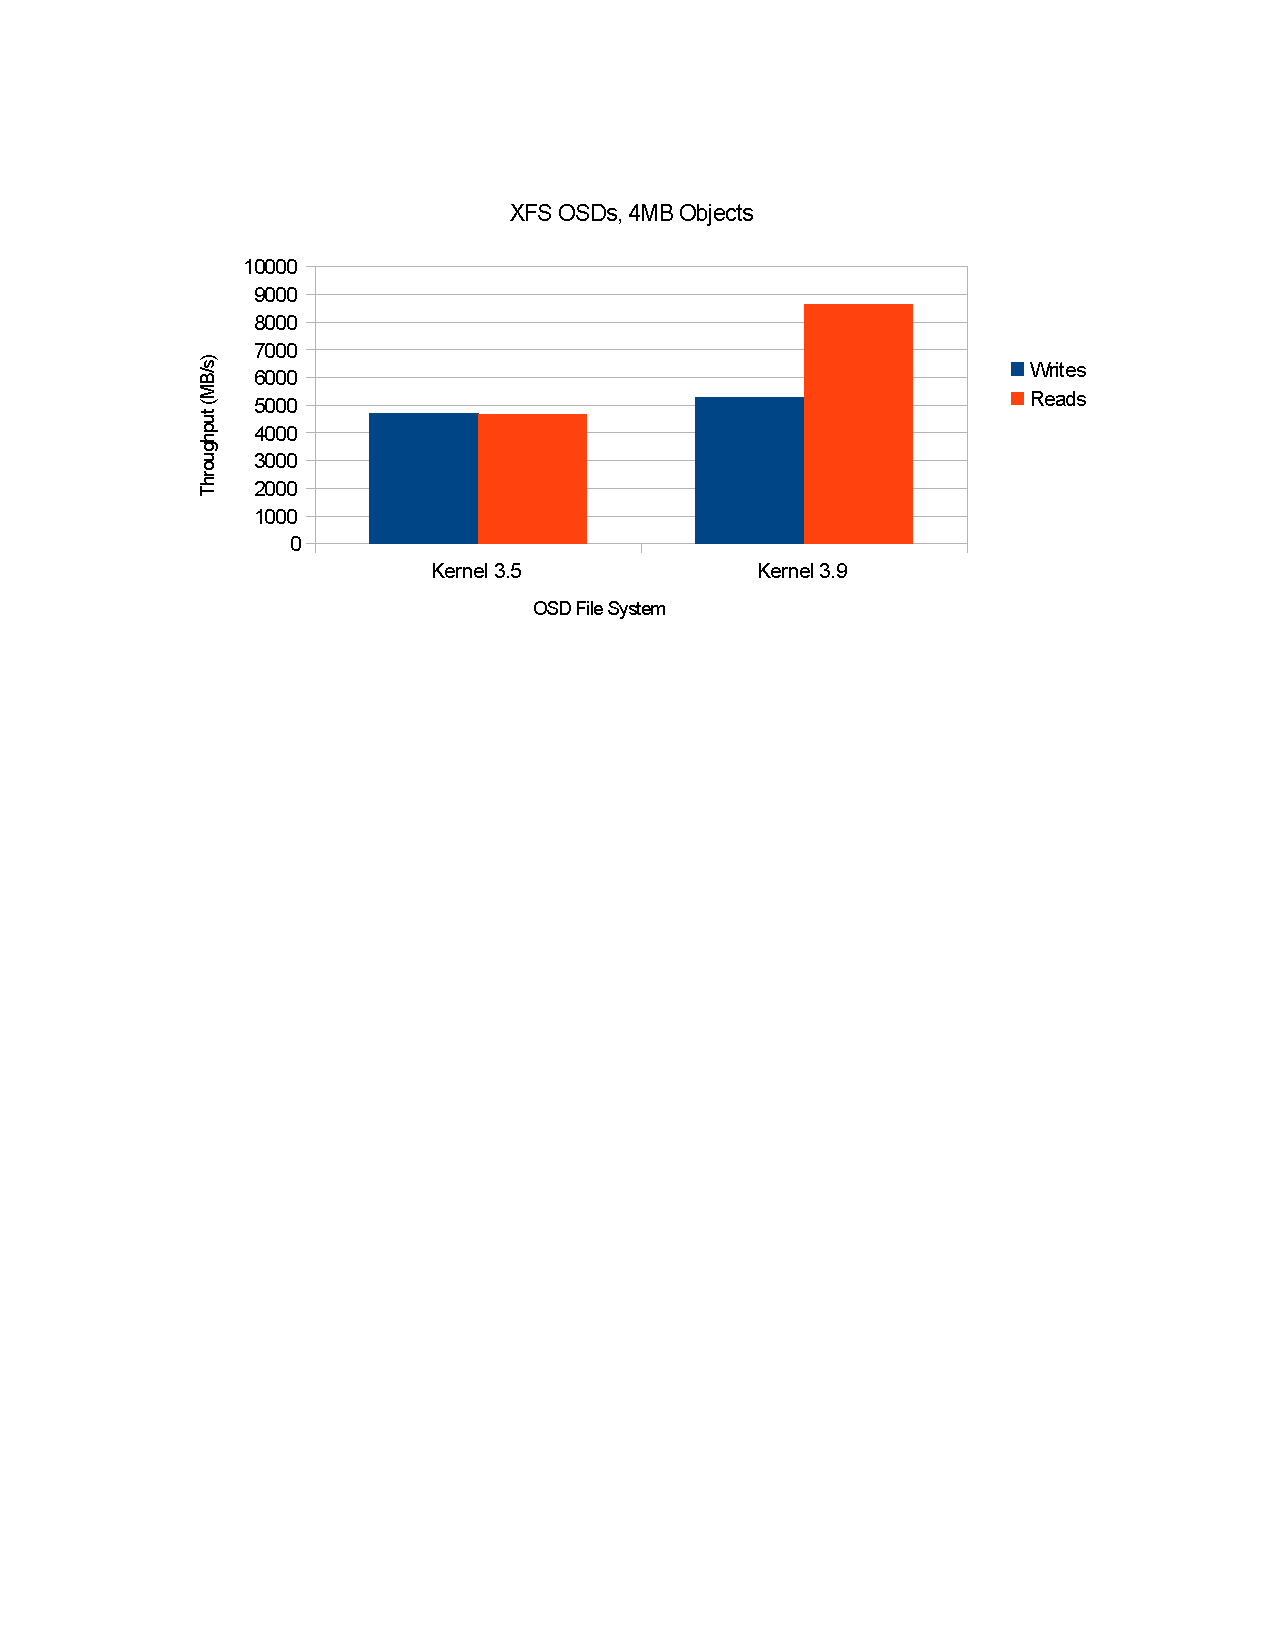
\includegraphics[width=4in]{rados-kernel-35vs39}
\caption{RADOS bench: Kernel 3.5 vs. 3.9}
\label{fig:rados-kernel}
\end{figure}



With the kernel changes writes performance improved slightly, while read
performance improved dramatically.  In addition to the kernel change, Sage Weil
suggested increasing the amount of read-ahead being performed by the CephFS
kernel client:

\begin{Verbatim}[samepage=true]
mount -t ceph 10.37.248.43:6789:/ /mnt/ceph -o
   name=admin,nocrc,readdir_max_bytes=4104304,readdir_max_entries=8192
\end{Verbatim}

%% SCOTT - is figure 15 IOR over Ceph and 14 is RADOS bench? If so, can we
%% mention that 15 shows the filesystem performance?

\begin{figure}[htb]
\centering
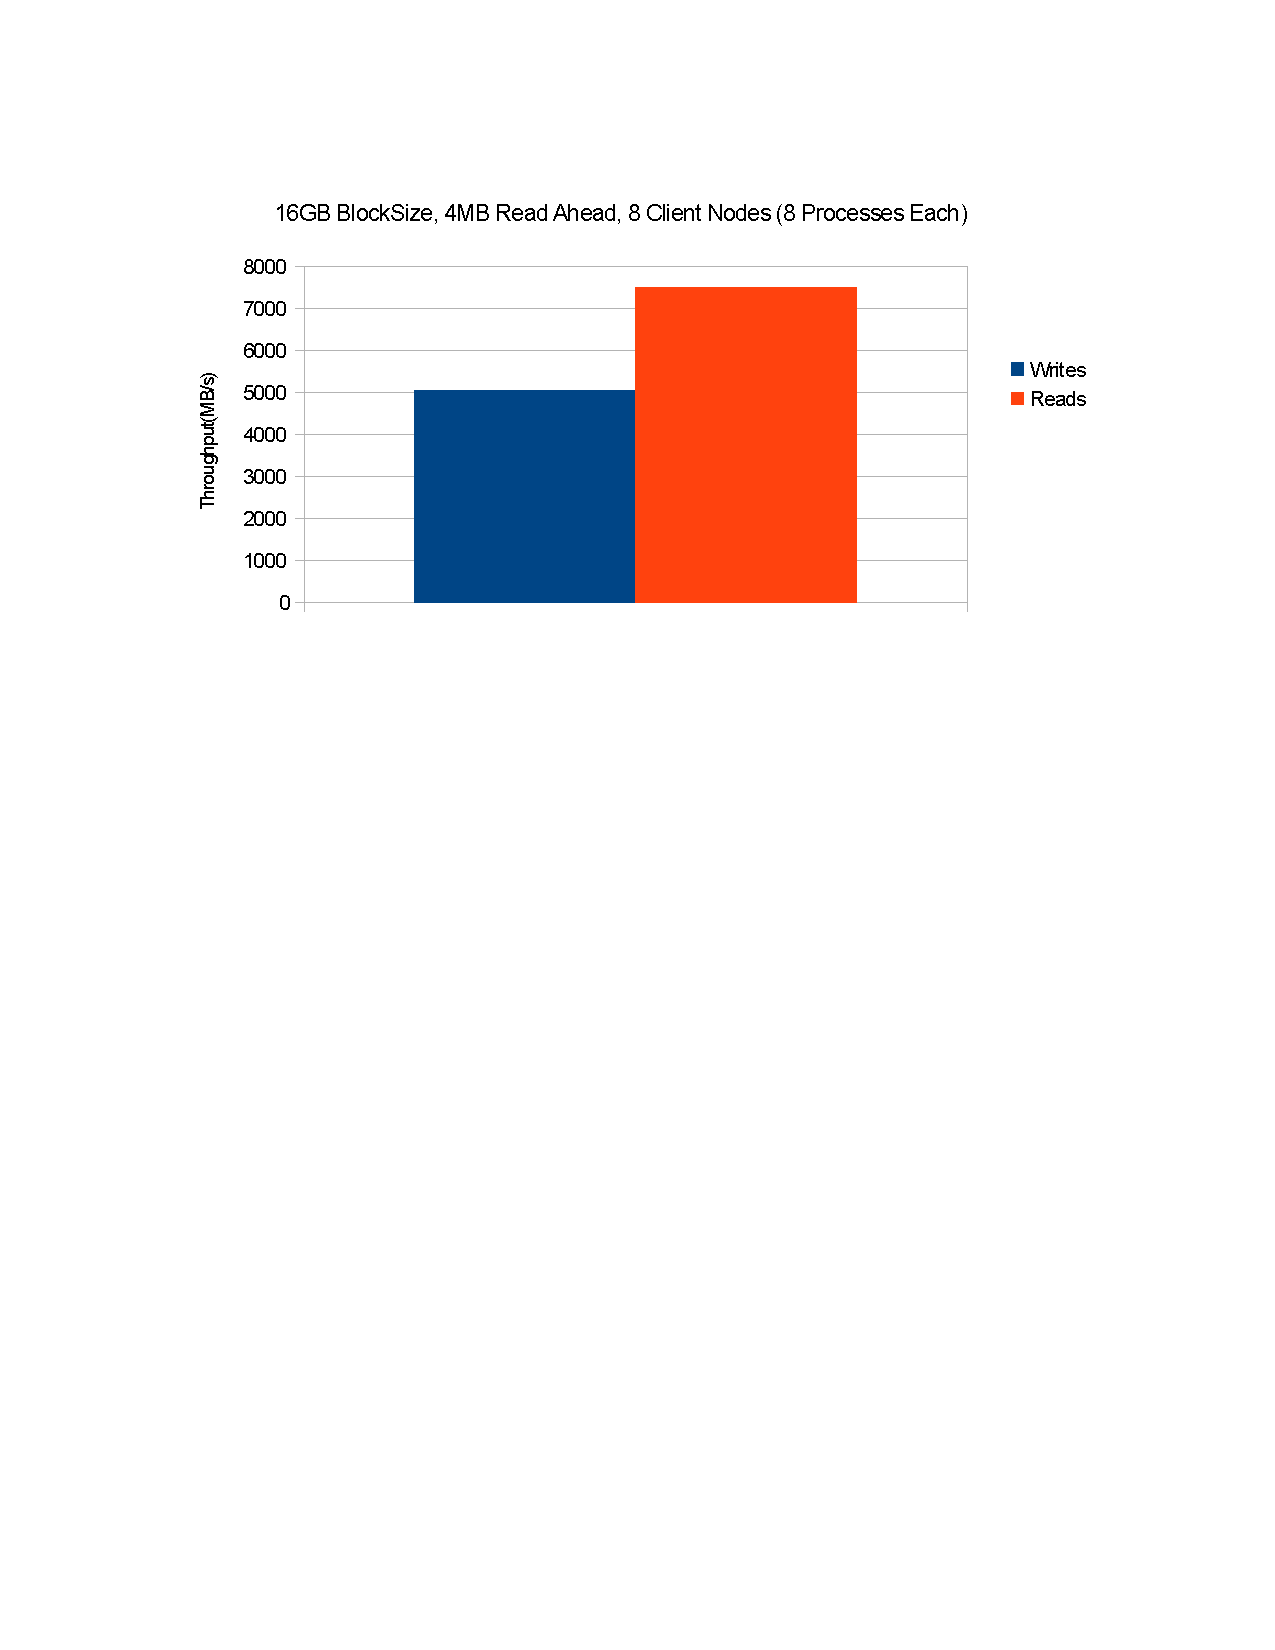
\includegraphics[width=4in]{ior-kernel-39}
\caption{CephFS performance with Kernel changes to 3.9, IOR with 4 MB transfer
size}
\label{fig:ior-kernel-39}
\end{figure}


By installing a new kernel, increasing read-ahead, and increasing the number of
client IOR processes, we were able to achieve a very satisfactory result on this
test run.


\subsection{Repeating IOR Scaling Test}

As before, we ran IOR scaling tests with two cases: transfer size 4 KB and 4 MB.
These results are illustrated in Figure~\ref{fig:ior-064}. As expected, we are
seeing a much improved picture of read and write performance, very much in
line with RADOS bench performance.

%% SCOTT - Can we use the same Y axis for these figures? Any comment from Inktank
%% as to why 4 KB performance is better than 4 MB performance?

\begin{figure}[htb]
\centering
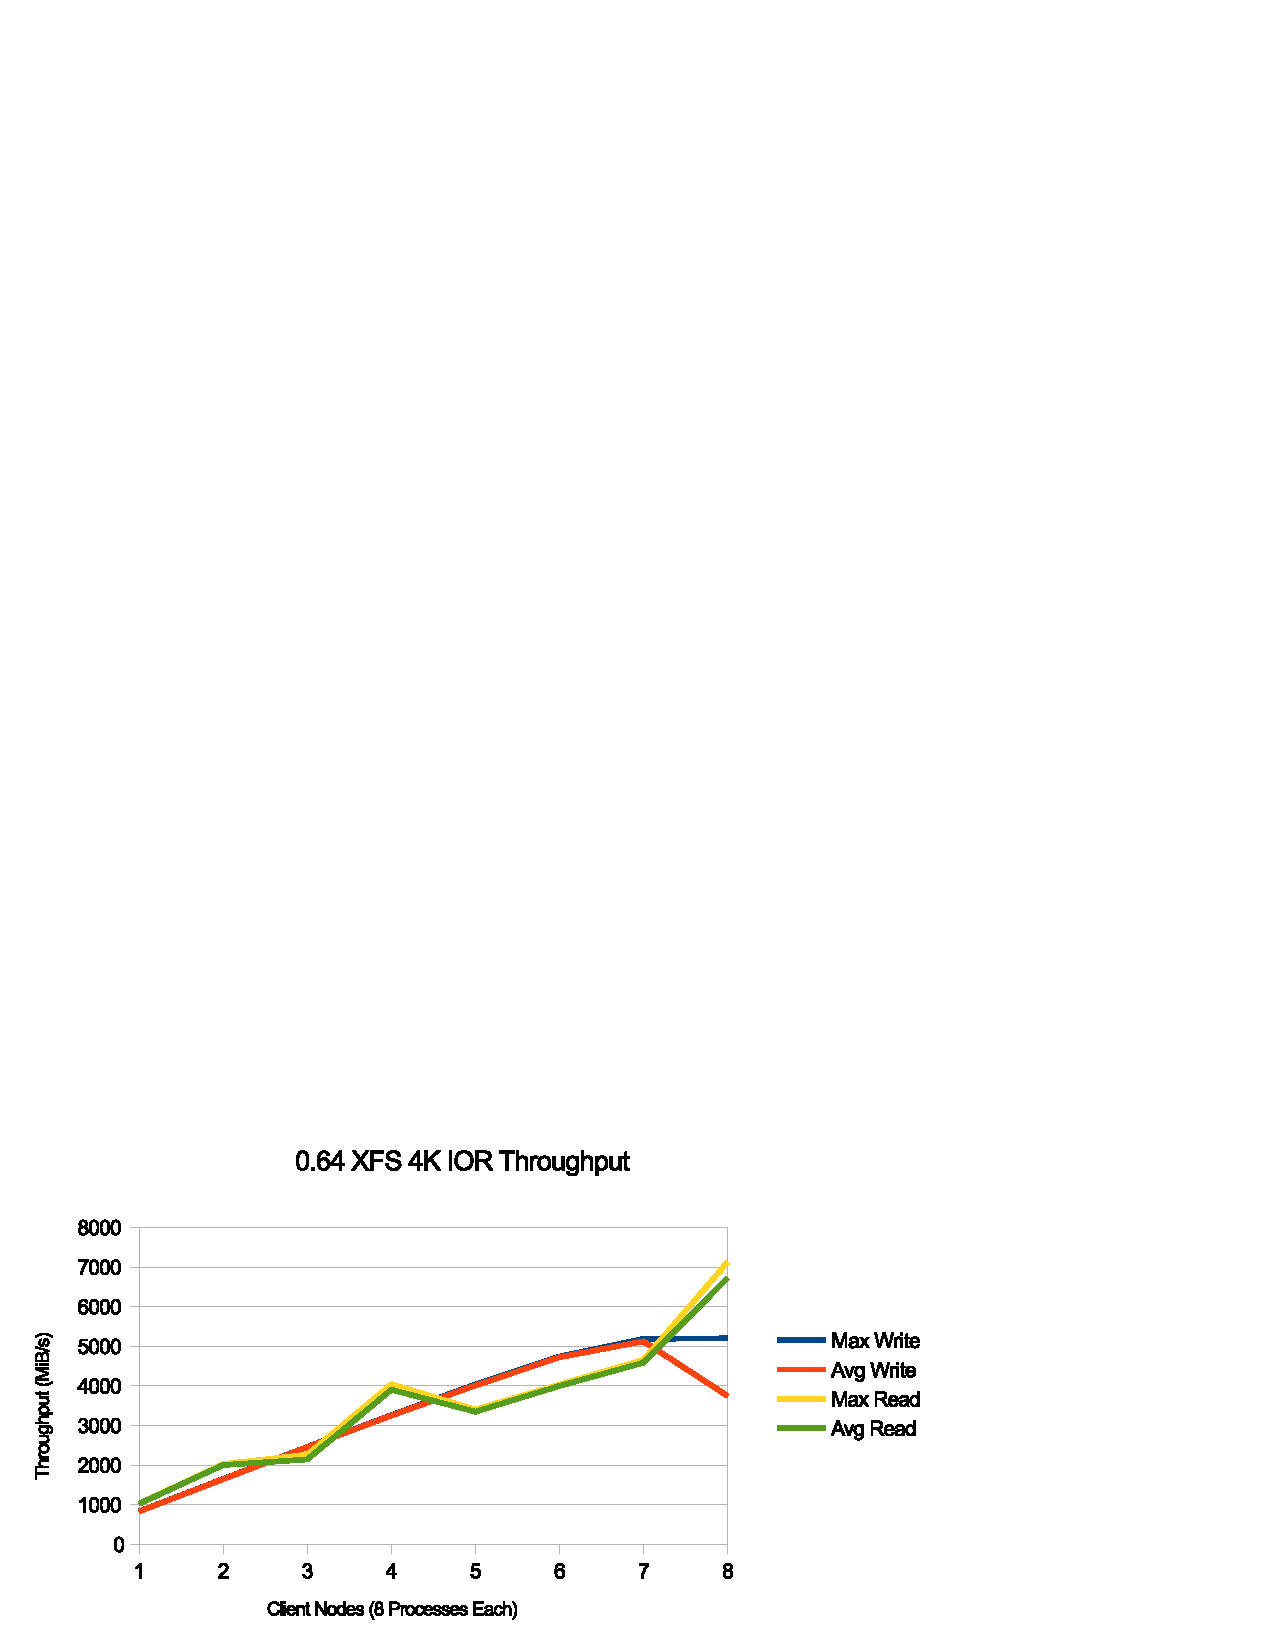
\includegraphics[width=5in]{ior-064-4k}
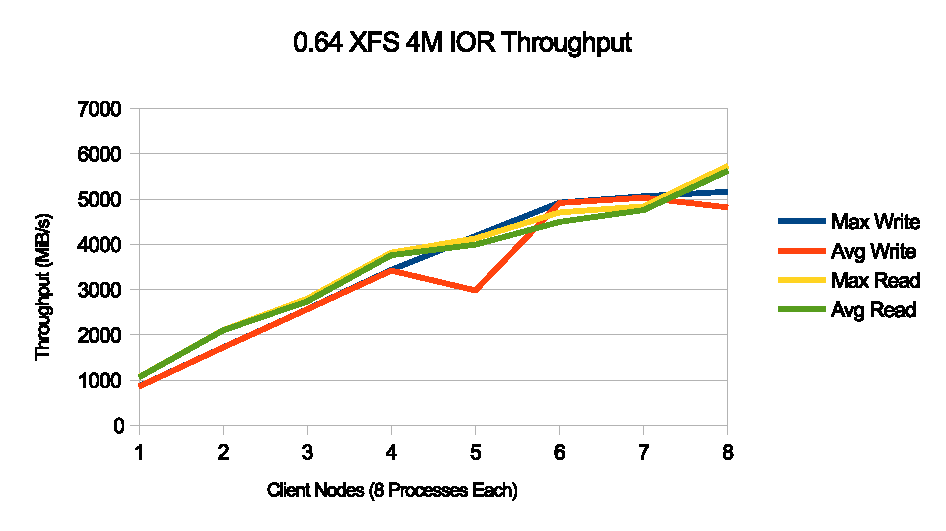
\includegraphics[width=5in]{ior-064-4m}
\caption{IOR Scaling Test: 4 KB and 4 MB transfer size}
\label{fig:ior-064}
\end{figure}

We observe a couple of places where the average write throughput is quite a
bit lower than the maximum.  This behavior was observed during other tests as well,
indicating that we may have periods of time where write throughput is
temporarily degrading.  Despite these issues, performance generally seems to be
improving as the number of clients increases.  Writes seem to be topping out at
around 5.2 GB/s (which is roughly what we would expect).  Reads seem to be
topping out anywhere from 5.6-7 GB/s, however it is unclear if read performance
would continue scaling with more clients and get closer to the 8 GB/s+ numbers we
saw with RADOS Bench.


\section{Metadata Performance}

\begin{figure}[htb]
\centering
%% -- 1st figure
\begin{minipage}[t]{0.5\linewidth}
\centering
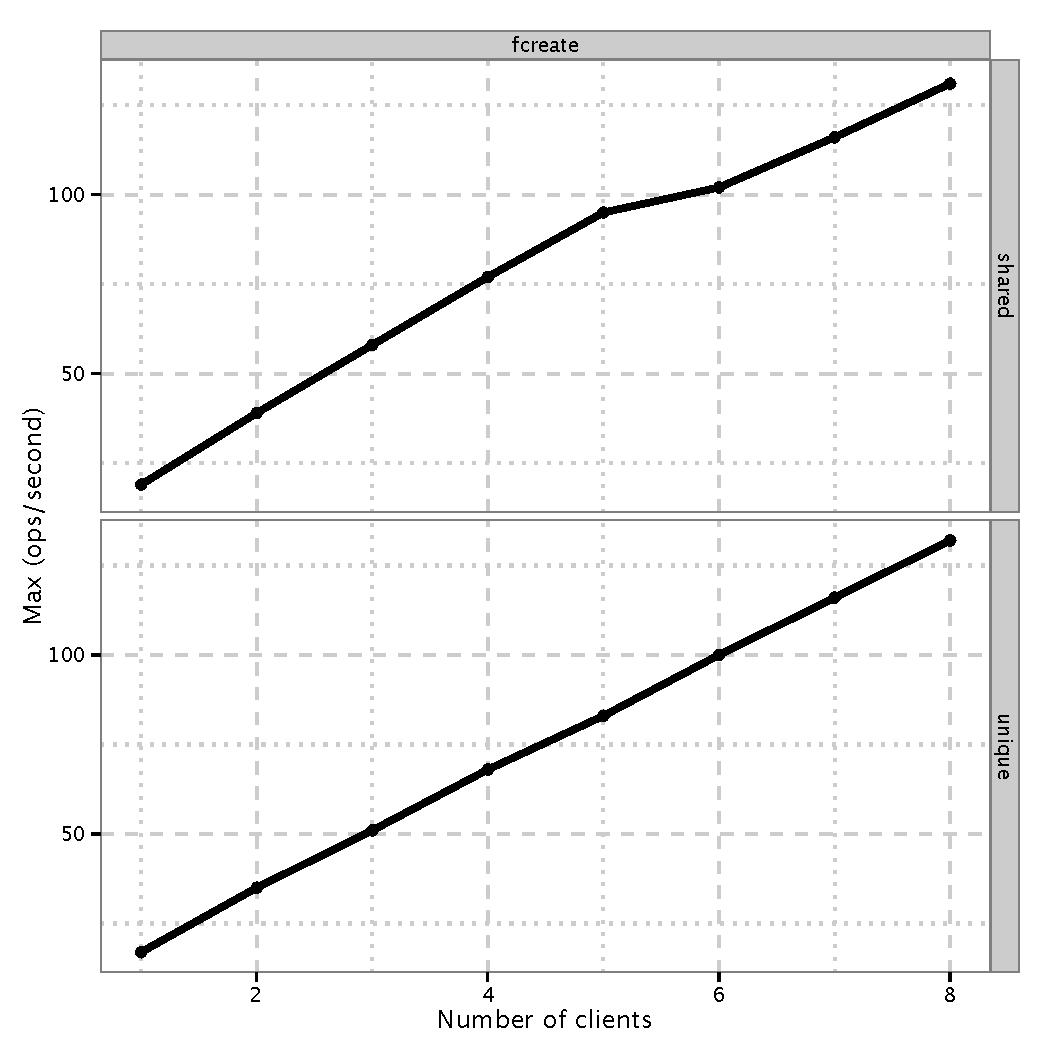
\includegraphics[width=3in]{data/mdtest-fcreate}
\caption{File creation vs.  number of clients}
\label{fig:mdtest-fcreate}
\end{minipage}%
\begin{minipage}[t]{0.5\linewidth}
\centering
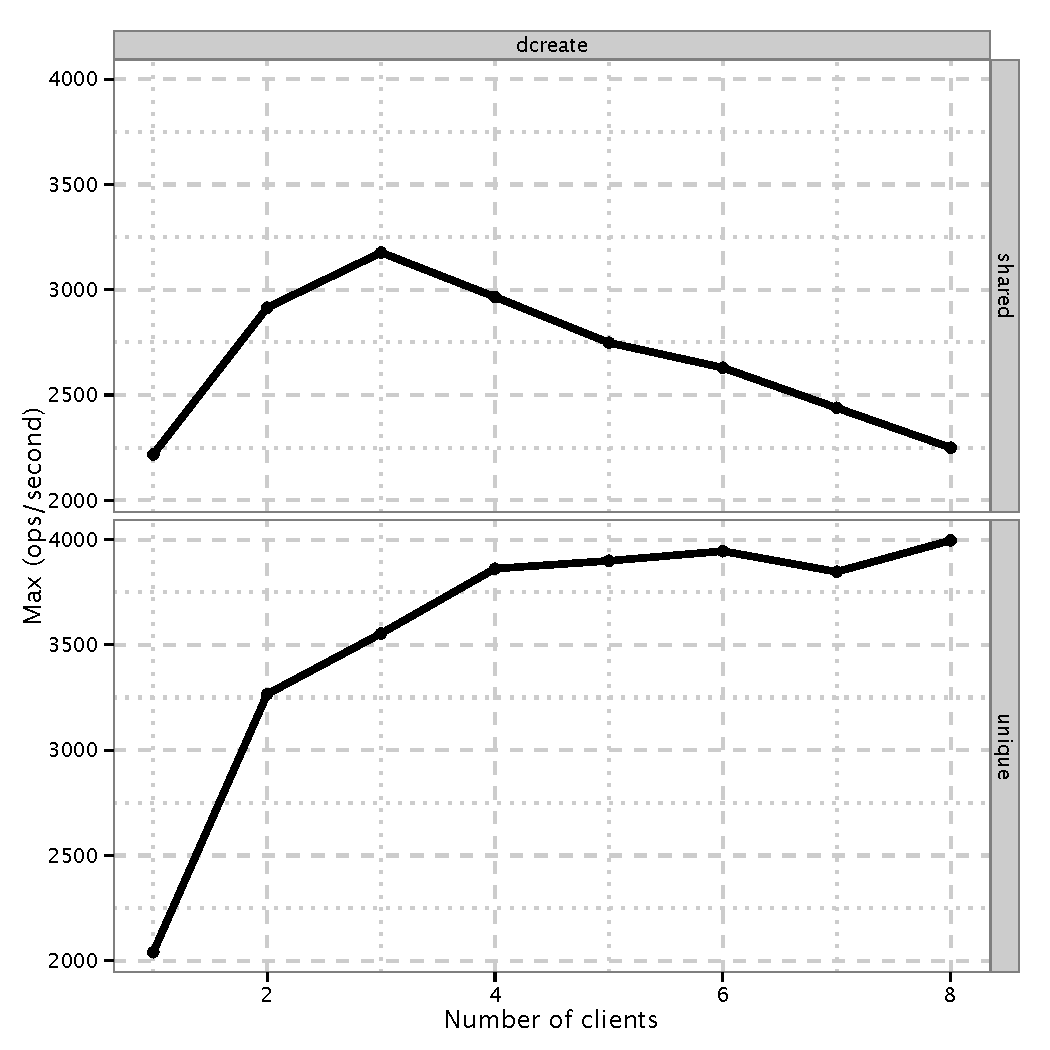
\includegraphics[width=3in]{data/mdtest-dcreate}
\caption{Directory creation vs. number of clients}
\label{fig:mdtest-dcreate}
\end{minipage}%
\end{figure}


In our particular setup, we have only one metadata server (MDS)
configured. Therefore, this is not a scalability test on the performance of
clustered MDS, which would be very interesting.
Instead, we focus on a single MDS, multiple clients (up to 8) and see how it
scales. The particular parameters we use for testing are:

\begin{itemize}
\item \verb!-w 1048576 -y!: for each created file, we write 1 MB data and
perform sync after it. This is a more realistic use case scenario than just
open, close and removal.

\item \verb!-n 1000!: this is per client file \textit{and} directories. For eight
clients, the number of files and directories is 8,000. Since we did not specify
either \verb!-D! or \verb!-F!, so this is a mixture of both.

\item \verb!-d /mnt/cephfs/tmp!: we do specify a directory, but unlike under
Lustre file system, where you can have single client multiple mounts (for
increasing workload per client), here we just give the test an explicit home.

\item \verb!-u!: without this option, we are exercising shared directory; with
this option, we are exercising unique directories.

\end{itemize}

Each test iterates five times and we are showing the max. 
We summarize the results as follows:

%Figure~\ref{fig:mdtest1c} is meant to give an overview on the trending of each
%directory (prefixed with d) and file (prefixed with f) operations, against the
%number of clients. Due to the scale difference, it doesn't convey the
%magnitude of lower numbers. 

\begin{itemize}

\item Within a single sharing mode (either shared or unique directory), the
directory stat and file stat, as well as file read exhibit strong linear
scaling property. 

\item While the other operations seems unaffected or flat by the number of
clients, it is not so if we zoom in, see \ref{fig:mdtest-fcreate} and
\ref{fig:mdtest-dcreate}:  as number of clients increases, we observed the
contention for shared directory. The performance degradation amount to 50\% or
more.

\item Though the same saturation or degradation trend is not observed for file
creation, it is likely due to we have not put enough of workload stress on MDS.

\end{itemize}


The results also show that file creation rate is signficantly lower than
directory creation rate. We stipulated two contributing factors: one is the file
creation is associated with 1 MB data write and followed by a fsync operation,
which is a rather heavy weight operation compare to directory creation. Another
factor is that we obtained above results from early version of Ceph without all
the tunings and improvement applied. Therefore, we repeated the same test on the
latest CephFS 0.64. The result is illustrated in
Figure~\ref{fig:mdtest-064-file-create}. As expected, we observed a significant
improvement on the file creation rate. We also note that as number of clients
increase, the file creation rate decreases rapidly, which suggested some form of
lock contention. This presents some interesting issues to be investigated
further.

\begin{figure}[htb]
\centering
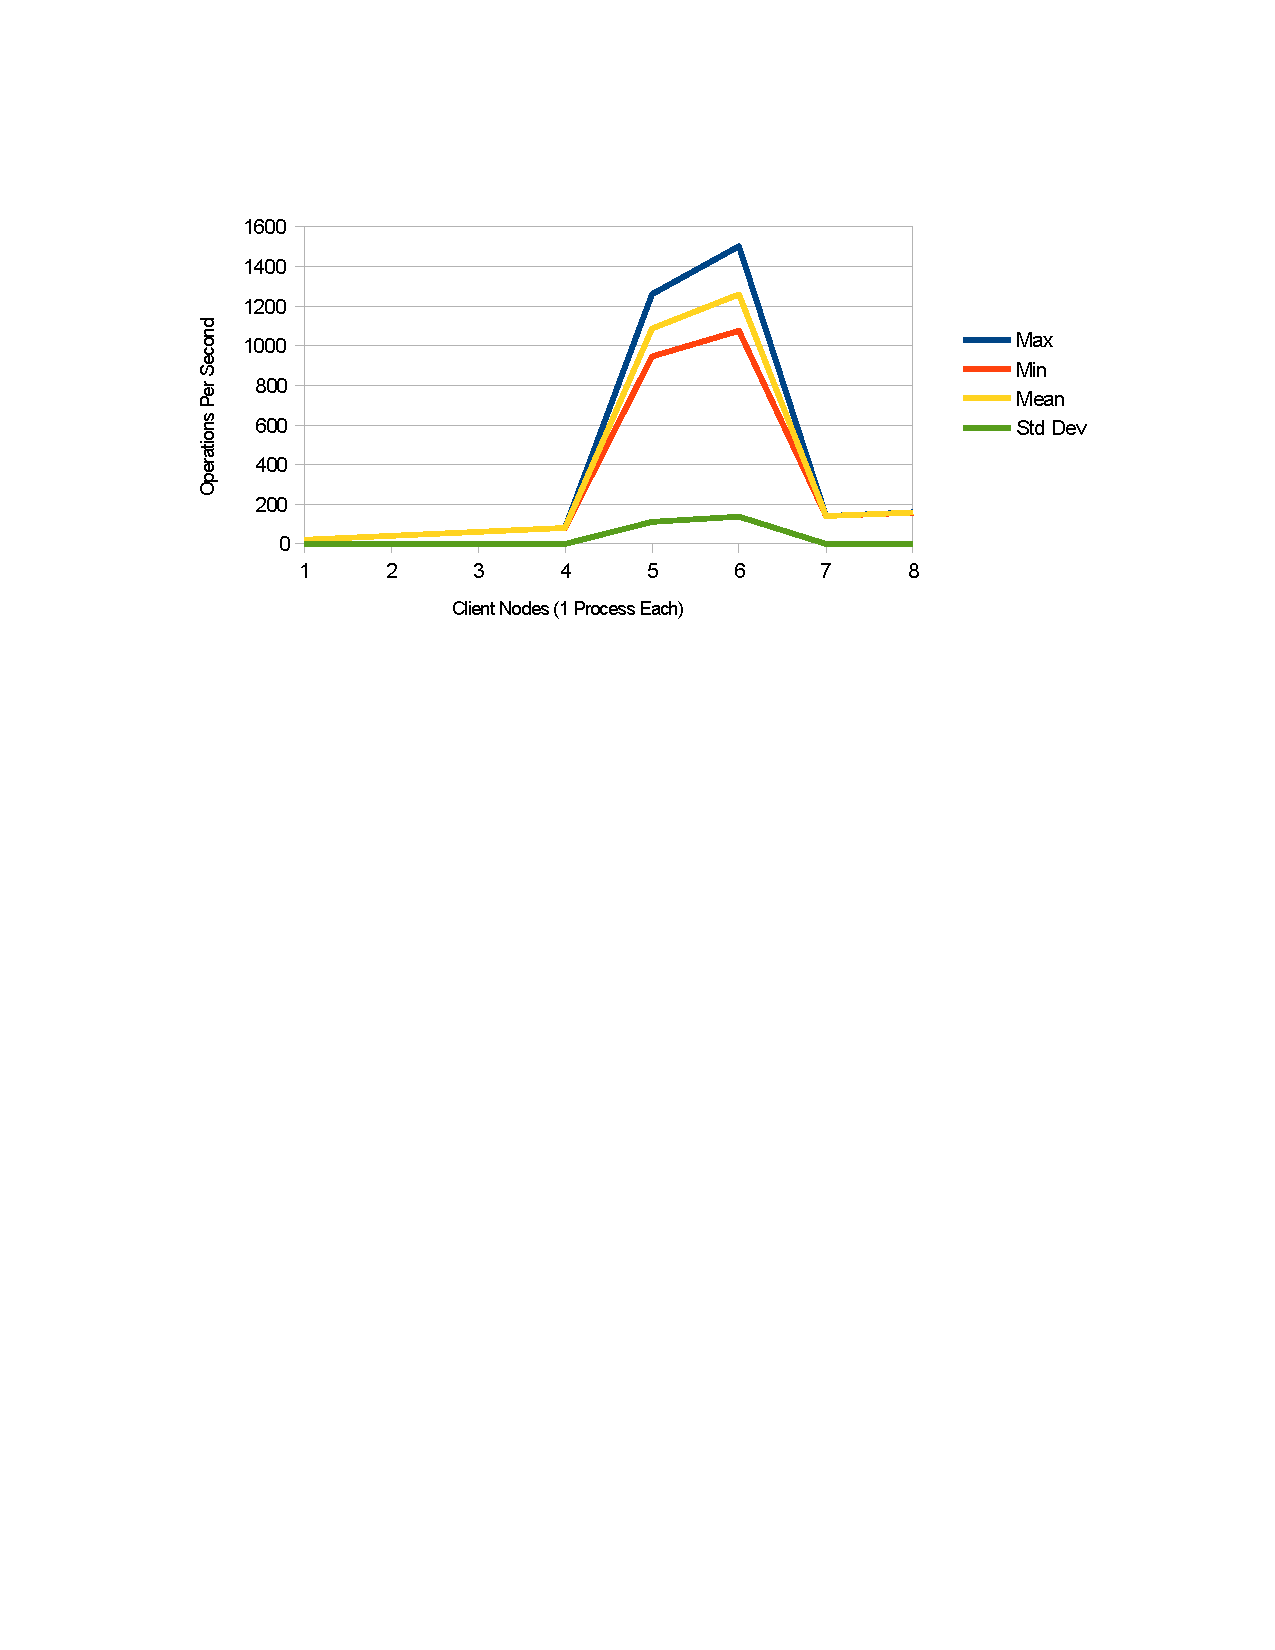
\includegraphics[width=4in]{mdtest-064-file-create}
\caption{mdtest of file creation on Ceph 0.64}
\label{fig:mdtest-064-file-create}
\end{figure}

\section{Observations and Conclusions}

This is preliminary observations from mostly performance perspective:

\begin{itemize}

  \item Ceph is built on the assumption that the underlying hardware components
  are unreliable, with little or no redundancy and failure detection capability.
  This is not the case in leadership computing facilities. We have disabled
  replication for pools, but this will take a toll somewhere in the processing
  and we do not know if this is significant.

  \item Ceph performs \textbf{metadata + data} journaling, which is fine for host
  system that has locally attached disk. However, this presents a problem in DDN
  SFA10-like hardware, where the backend LUNs are exposed as block device
  through SCSI Request Protocol (SRP) over IB. The journaling write requires twice the bandwidth
  compare to Lustre-like metadata-only journaling mechanism. For Ceph to be
  viable in this facility, we will need to address this.

  \item We observed consistent results and linear scalability at the
  RADOS level. However, we did not observe the same at the file system level with synthetic
  benchmark suites such as IOR. We have experienced large performance swings
  during different runs, very low read performance when transfer size is small,
  and I/O errors tend to happen when system is under stress (more clients and
  large transfer sizes). These are not particularly reproducible results, but it
  suggests that there are opporunities for code improvement and maturation.

\end{itemize}

\section*{Appendix A - CephFS Final Mount Command}
\addcontentsline{toc}{section}{Appendix A - CephFS Final Mount}

\begin{Verbatim}
mount -t ceph 10.37.248.43:6789:/ /mnt/ceph -o
      name=admin,nocrc,readdir_max_bytes=4104304,readdir_max_entries=8192
\end{Verbatim}


\section*{Appendix B - OSD File System Options}
\addcontentsline{toc}{section}{Appendix B - OSD File System Options}

\input{osd_fs.txt}

\section*{Appendix C - CRUSH Map}
\addcontentsline{toc}{section}{Appendix C - CRUSH map}

This crush map is just an example of full OSD mapping. As we create and
re-create different testbed subests with different OSD configurations, the map will
change accordingly.

\input{crush.txt}


\section*{Appendix D - Final ceph.conf}
\addcontentsline{toc}{section}{Appendix D - Final ceph.conf}

\input{ceph-short.txt}

\section*{Appendix E - Tuning Parameters}
\addcontentsline{toc}{section}{Appendix E - Tuning Parameters}

For parameter sweep, here are the settings we iterated through.  Some of these
are "compound" settings where we increased or decreased multiple things in the
ceph.conf file at the same time to reduce the number of permutations that would
need to be tested.

\input{tuning.txt}

\end{document}
